% File name: report/report.tex

\begin{filecontents}{bibliography.bib}
@ONLINE {toastersmd,
    url= {http://openhardware.net/Misc_Stuff/ToasterSMD/},
    urldate = {2014-05-12},
    author = {Tom Walsh},
    title = {ToasterSMD}}
    
@ONLINE {hotplate,
	url = {http://www.hobbytronics.co.uk/hotplate-smd-soldering},
	urldate = {2014-05-12},
	author = {Hobbytronics},
	title= {Hotplate Surface Mount SMD Soldering Tutorial}}
	
@ONLINE {github,
	url = {https://github.com/JamesGlanville/pcb2gcode-metric},
	urldate = {2014-05-12},
	author = {James Glanville},
	title = {JamesGlanville / pcb2gcode-metric}}
	
@ONLINE {imodela,
	url = {http://www.imodela.co.uk/},
	urldate = {2014-05-12},
	author = {TechSoft UK Limited},
	title = {iModela, the smart compact milling / engraving machine.}}
	
@ONLINE {caliperdata,
	url = {http://www.robotroom.com/Caliper-Digital-Data-Port.html},
	urldate = {2014-05-12},
	author = {David Cook},
	title = {Interfacing with Digital Calipers}}
	
@ONLINE {fpga4fun,
	url = {http://www.fpga4fun.com/SMD.html},
	urldate = {2014-05-12},
	author = {Jean P. Nicolle},
	title = {SMD (Surface Mount Device) / SMT (Surface Mount Technology)}}
	
@ONLINE {smdwiki,
	url = {http://en.wikipedia.org/wiki/Surface-mount_technology},
	urldate = {2014-05-12},
	author = {various},
	title = {Surface-mount technology}}
	
@ONLINE {excel2latex,
	url = {http://ericwood.org/excel2latex/},
	urldate = {2014-05-22},
	author = {Eric Wood},
	title = {excel =\textgreater LaTeX}}
	
@ONLINE {thingipaste,
	url = {http://www.thingiverse.com/thing:20733},
	urldate = {2014-05-22},
	author = {Richard Horne},
	title = {Universal Paste Extruder for 3d printers}}
\end{filecontents}

\documentclass[a4paper,11pt]{article}  % Standard document class
\usepackage[english]{babel}            % Set document language
\usepackage{fullpage}                  % Set up page for small margins etc
\usepackage{listings}
\usepackage{graphicx}                  % For including images in document

\usepackage{tikz}
\usetikzlibrary{shapes,arrows}

\usepackage{appendix}
\usepackage{color}
\usepackage{hyperref}

\usepackage{caption}
\usepackage{subcaption}

\usepackage{biblatex}
\addbibresource{bibliography.bib}

\usepackage[xindy,toc]{glossaries}
\makeglossaries

\newglossaryentry{GCODE}
{
	name=GCODE,
	description={A human-readable numerical control programming language, commonly used in CNC machines}
}

\newglossaryentry{PCB}
{
	name=PCB,
	description={Printed circuit board. A circuit board made of an insulating sheet covered in conductive traces to which components are soldered. FR-4 is the common grade
			of glass-reinforced epoxy used in most PCBs, and as such is the only material covered by this project.}
}

\newglossaryentry{SMD}
{
	name=SMD,
	description={Surface mount device. A component with no through-hole leads which is designed to be soldered to a PCB. In some cases the components are glued to the board
			for strength.}
}
\newglossaryentry{THT}
{
	name=THT,
	description = {Through-hole technology. An older technology (compared to SMD) where component leads are inserted into holes in a PCB. Still used in cases where the superior 
			attachment strength in required.}
}
\newglossaryentry{CNC}
{
	name=CNC,
	description = {Computer numerical control. Refers to the automation of machine tools with programmed commands.}
}

%\usepackage{placeins}                  % Allows use of \FloatBarrier
% to avoid images or tables
% moving into next section
%\usepackage{subfig}                    % For subfigures...

\usepackage{amsmath}                   % For improving maths/formula typesetting
%\usepackage{tabular}                  % Table changing package

%\usepackage{algpseudocode}             % For producing algorithms/flowcharts

\usepackage{listings}                  % For including source code in document
\lstset{
  basicstyle = \small
}

% Provide command for scientific notation
\providecommand{\e}[1]{\ensuremath{\times10^{#1}}}
\providecommand{\degrees}{\ensuremath{^{\circ}}}

% Define title here:
\title{4th Year Project: Automated soldering/solder paste machine (C-PJGL2-7)} %C-PJGL2-7
\author{James Glanville}
\date{11th June 2013}

\hypersetup{
    colorlinks,
    allcolors=blue,
    linktoc=all,
}

\begin{document}

% generate title
\maketitle

\begin{figure}[ht!]
\centering
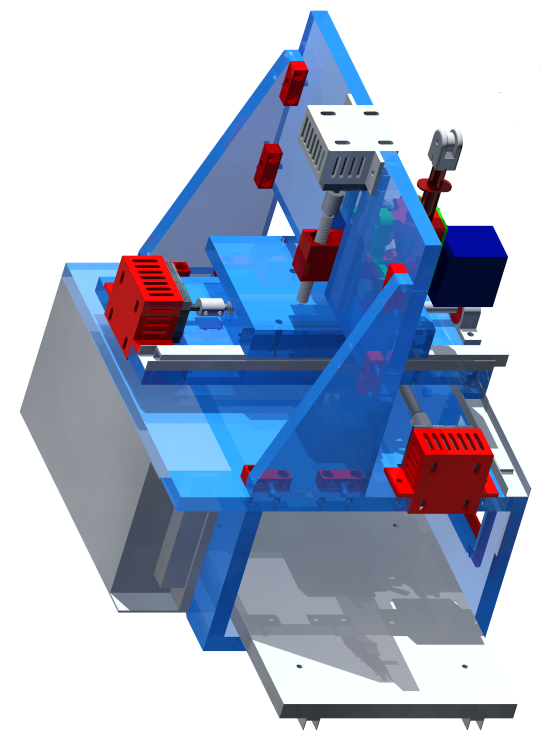
\includegraphics[width=100mm]{resources/render.png}
\label{render}
\end{figure}

\newpage
\tableofcontents

\newpage

\section{Introduction}

\begin{figure}[ht!]
\centering
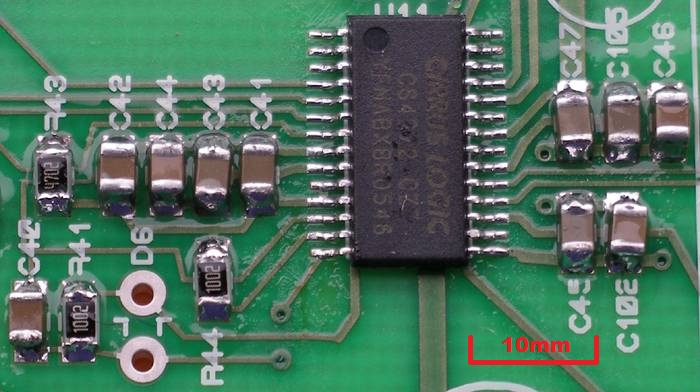
\includegraphics[width=120mm]{resources/smt_soldering.jpg}
\caption{Example surface mount board.}
\label{smdexample}
\end{figure}

The aim of this project is to develop ways to assist electronics hobbyists in working with SMD electronic components
and circuit boards (See Figure \ref{smdexample}). \gls{SMD}s are electronic components which are designed to be soldered to \gls{PCB}s
(Printed Circuit Boards) without requiring holes to be drilled in the board. Compared to \gls{THT}(Through-hole technology), SMD parts 
are usually smaller and cheaper and as a result are becoming ubiquitous in many applications. Even when hobbyist users do
not require the size or cost advantages, many modern devices are only available in SMD packages. Using SMD parts require
smaller board features (A manufacturing challenge) as well as more advanced soldering techniques. For this project, a machine
is envisioned which solves some or all of the challenges involved to ease the process of SMD board development.

\vspace{0.5cm}
As an example of the need for such a machine, see Figure \ref{usbisolator}. A USB isolator was required (to make USB connections to devices with non-isolated
power supplies), which uses an ADUM3160 SOIC-28 part (See full schematic, Figure \ref{usbisolatorschem}). Without an automated method of board manufacture, the
traces were hand drawn in etch-resist on each side of a double-sided board, and manually soldered all SMD parts. This was slow, and as figure \ref{usbisolator} shows, does not give
neat results.


\begin{figure}[ht!]
\centering
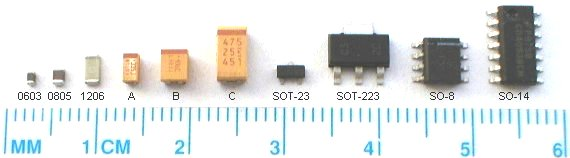
\includegraphics[width=150mm]{resources/SMDsizes.jpg}
\caption{Example SMD components (From \cite{fpga4fun})}
\label{overflow}
\end{figure}

\begin{figure}[ht!]
\centering
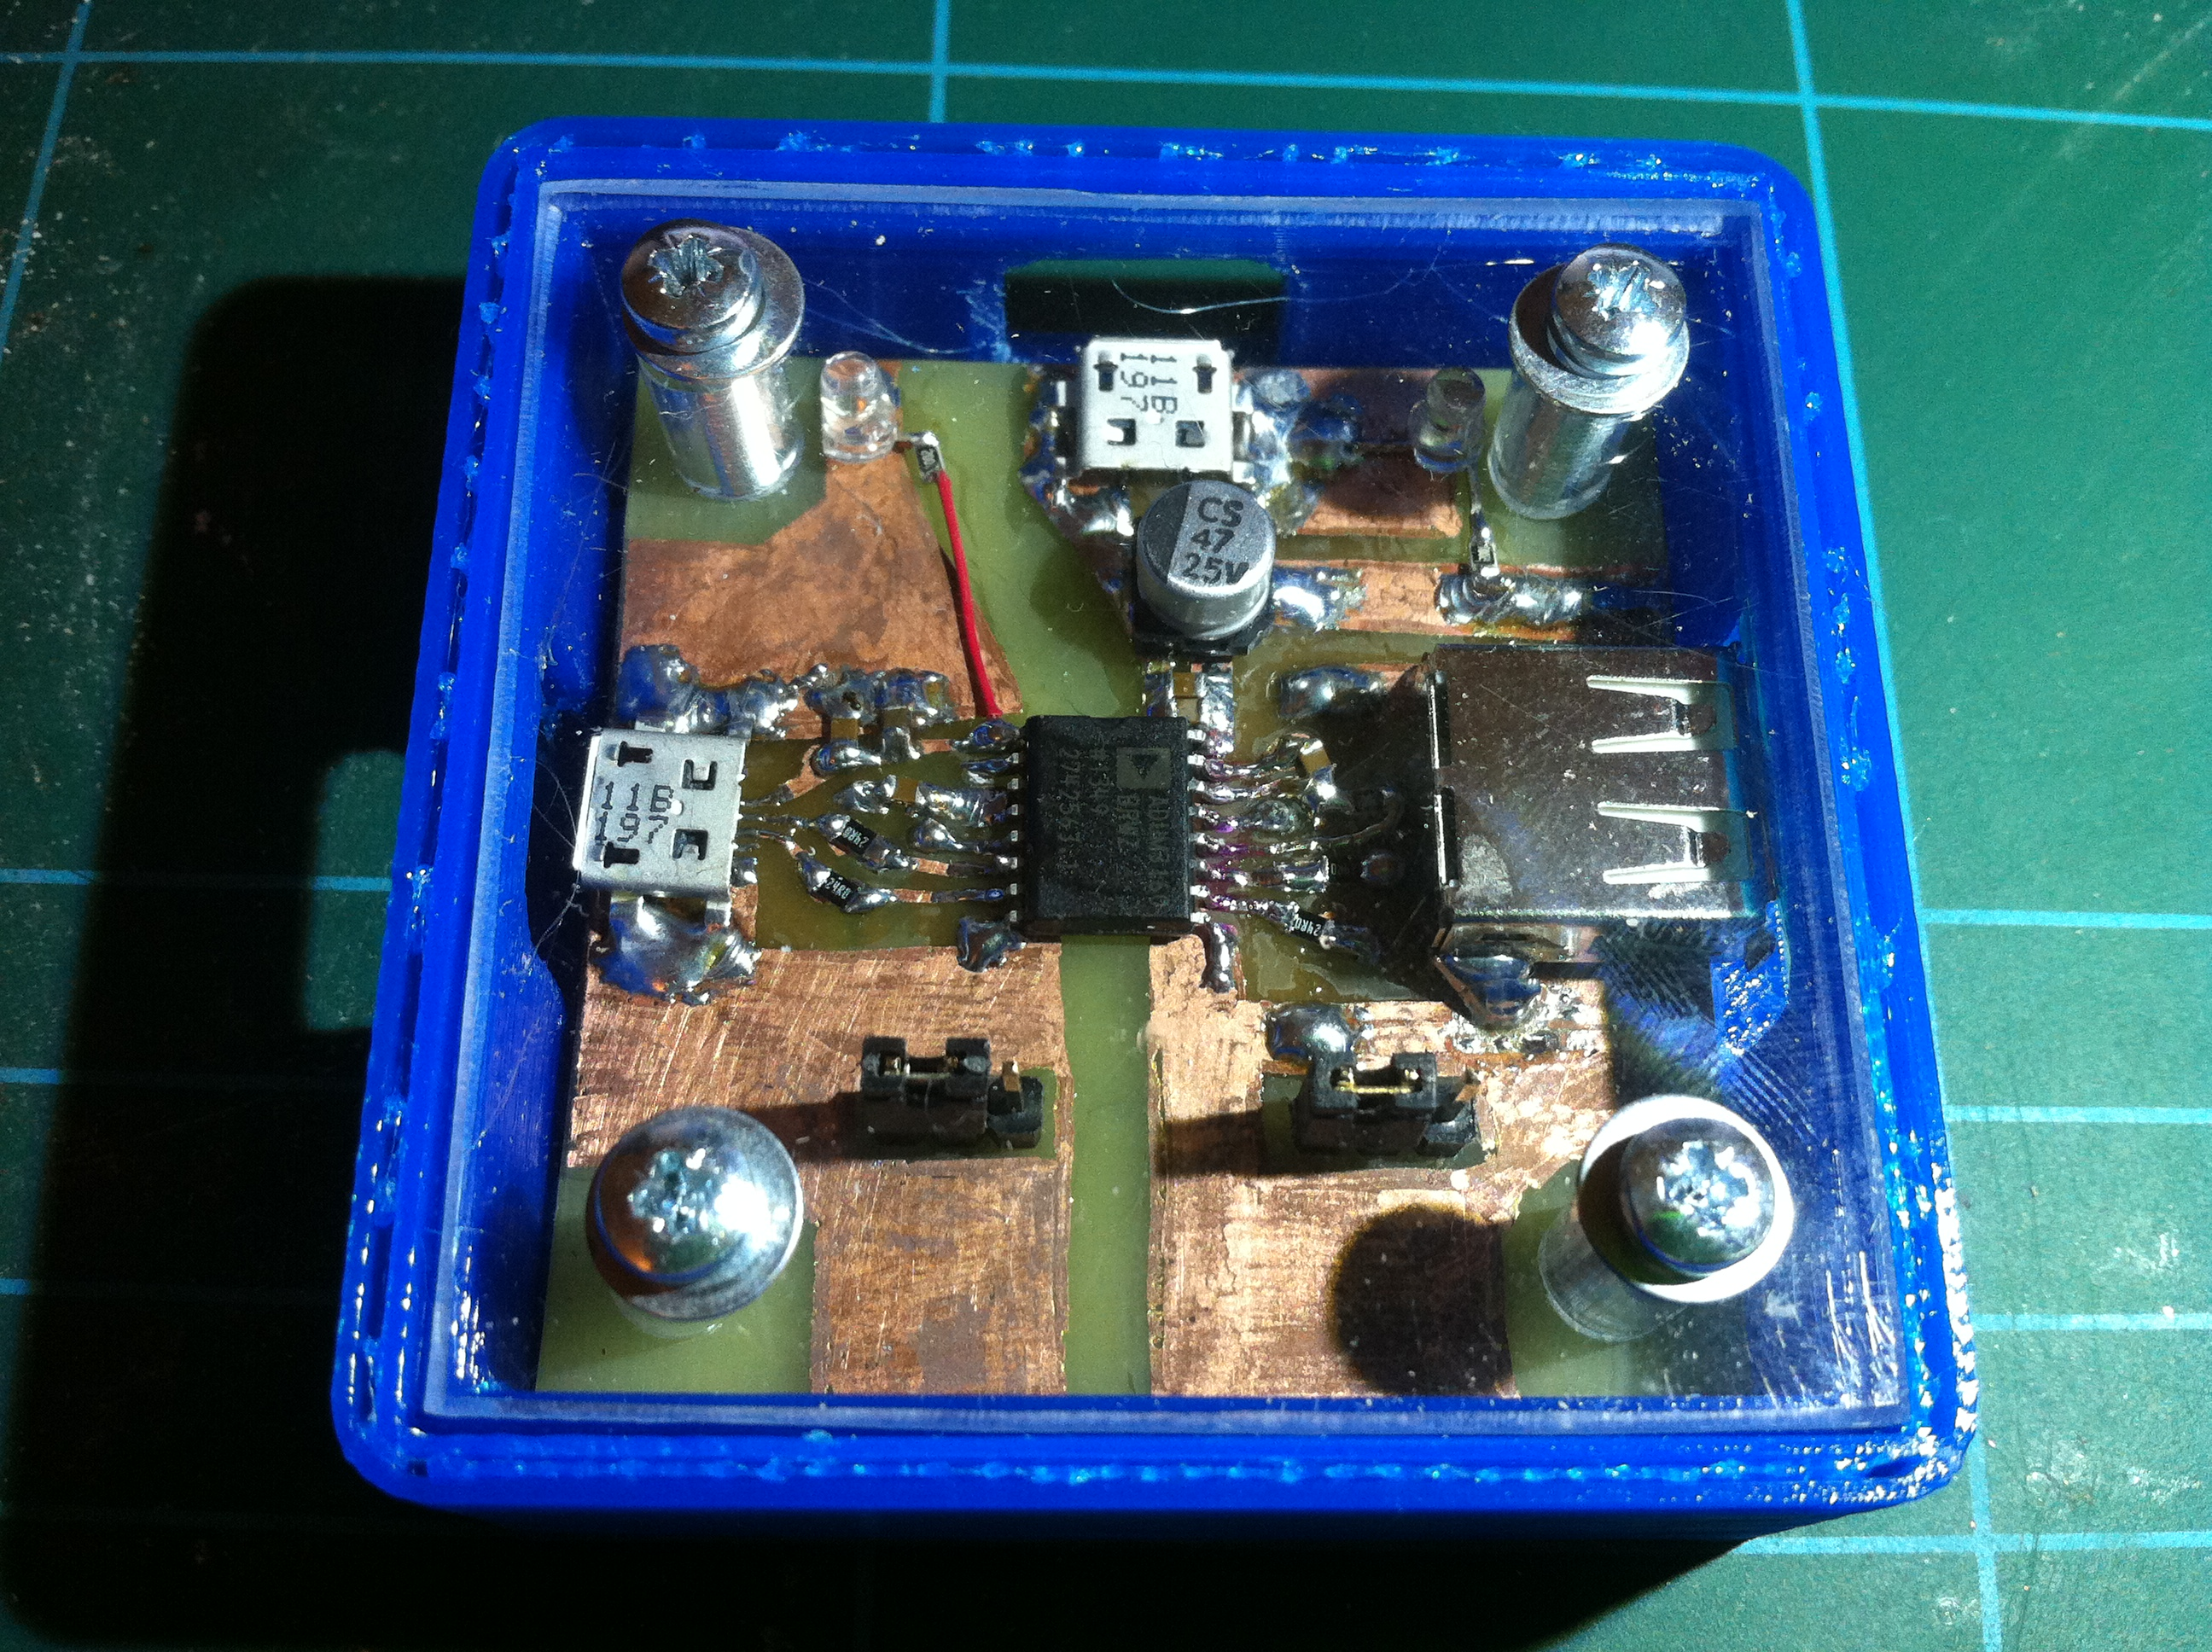
\includegraphics[width=120mm]{resources/usbisolator.jpg}
\caption{My USB isolator.}
\label{usbisolator}
\end{figure}

\begin{figure}[ht!]
\centering
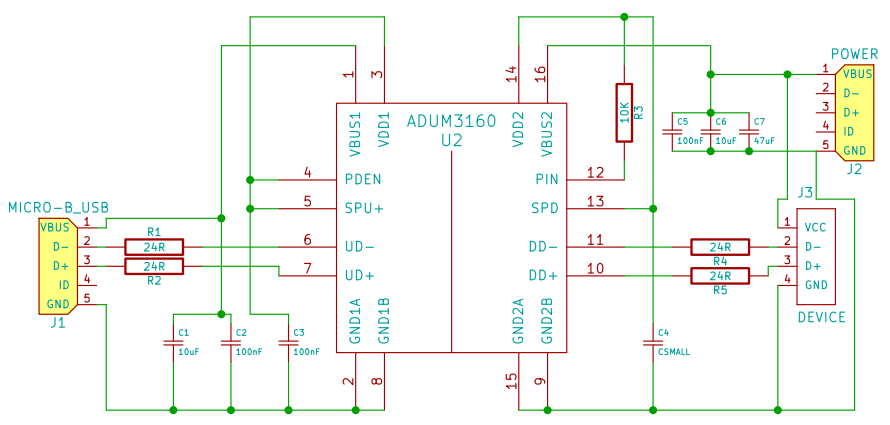
\includegraphics[width=120mm]{resources/isolatorschem.png}
\caption{USB isolator schematic.}
\label{usbisolatorschem}
\end{figure}

\section{Existing Solutions}
There are a number of hobbyist solutions to deal with SMD parts:

\subsection{Hand soldering}
Despite the increased complexity, many SMD parts can be soldered by hand. There are three main methodologies for this process:

\begin{itemize}
	\item	The pins are soldered individually. This is mainly suitable for larger SMD parts. A steady hand is required, as well as good eyesight.
			Binocular microscopes are often used to assist this process.
	\item	The process of "drag soldering" is used. The device is placed on the board, and a small amount of solder is placed on the tip of a soldering iron.
			The iron is slowly "dragged" along the pins. If done correctly, surface tension effects cause the majority of the solder to remain on the tip of the iron,
			while the necessary electrical connections are soldered.
	\item	The pins are roughly soldered, making sure each pin is at least soldered to the board. Many short circuits between adjacent pins will be present. Solder wick
			is then used with copious flux to remove excess solder between pins.
\end{itemize}

These methods are imprecise, and will often necessitate the use of solder wick or a solder sucker to remove solder bridges (See Figure \ref{handsolder}). More importantly, they are wholly unsuitable
for use with "leadless" packages. Instead of metal pins, these devices only have metal pads on their bases. Without exposed metal when the device is placed, it is not possible
to solder the connections by hand.

\begin{figure}[ht!]
\centering
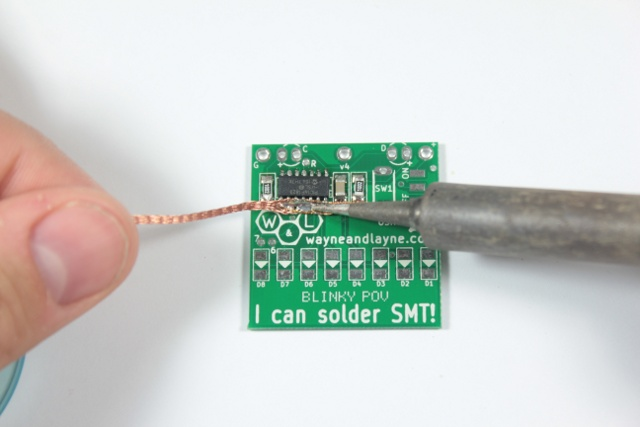
\includegraphics[width=120mm]{resources/handsoldering.jpg}
\caption{Removing excess solder with solder wick.}
\label{handsolder}
\end{figure}

\subsection{Solder paste}

Solder paste consists of powdered metal solder suspended in flux. It is used commercially to manufacture boards with SMD components. The solder paste is applied to the board where
connections are to be made. The devices are then placed on top (the paste has slight adhesive properties which limits undesirable component movement). Finally the paste is heated either directly
or indirectly which causes it to melt and form solder joints. The paste is placed in a number of ways:

\begin{itemize}
			\item	Solder stencils: A thin stencil is manufactured, usually from Mylar (trade name for BoPET) or stainless steel. It has holes which correspond to locations on the board that require solder.
					Solder paste is then roughly applied to the top of the stencil before being scraped off. This forces controlled volumes of paste into the holes.
					This a very quick process, and suitable for production quantities, but has the expensive set-up costs of stencil manufacture.
			\item	Solder paste can be applied by hand using a syringe. However, this requires high accuracy while placing paste and is time consuming.
			\item	Automated solder paste extrusion uses a CNC (Computer Numerical Control) platform to manoeuvre a solder paste extruder around the board. Small amounts of paste
					are extruded where necessary. This is not the fastest method of manufacture, but is suitable when only small numbers of boards are required.
\end{itemize}

Once the solder paste has been placed and the devices placed on top, it must be heated to form solder connections. This can be achieved in several ways:

\begin{itemize}
			\item	A hot air gun can be used manually to locally heat the required areas of the board. Hot air guns are inexpensive, but the process requires care so as not to overheat any
					components. It can also be relatively difficult to get the correct temperature profile - some solder joints may be overheated while some may not fully form.
			\item	Entire board heating involves placing the board in an oven which is heated to the correct temperature. This can vary from large commercial equipment to the use of a
					converted toaster oven.
\end{itemize}
			
\section{Project Idea}
It was decided to approach the project by building a machine which can extrude solder paste accurately, and then place
the surface mount devices on top. It should achieve this with minimal human interaction. The machine should also be able to
drill holes for through-hole devices, as well as be equipped with a milling bit for isolation routing through copper-clad PCBs.

\parskip 0.18in

When finished, the machine should be able to be connected to a computer via a USB port. A custom GUI will load the necessary 
design files (for example the holes to be drilled, pads to be soldered), generate the necessary GCODE, and send it to the printer.

\section{Requirements}

\subsection{X/Y axes}
A device pitch of 0.4mm (distance from centre of one pin to the next) is on the lower end of SMD ICs. Using solder paste,
devices will shift slightly upon heating to self-align. A requirement is that the device should be placed to a
small fraction of its pitch, so there is no danger of incorrect connections. An accuracy of $\pm$ 0.05mm
in placement was chosen as a project goal. This should be sufficient to ensure the correct connections are made, but may be difficult to achieve in practice.

\subsection{Board size}
A maximum board size of 100x100mm would be sufficient for the vast majority of boards. 100x100mm was chosen because that
is the maximum board size using the free version of EAGLE, a popular design package. As a result, there are a lot of designs
that use the maximum size, and it would be useful if this project allowed those designs to be populated.

The PCBs needed for the IDP fit within the 100x100mm area.

\subsection{Rigidity}
The sideways forces generated by the isolation routing bits were measured to be less than 2N. It is important that the $\pm$ 0.05mm
accuracy requirement is met under this condition.

\section{Design}

\subsection{X/Y axes}

The X/Y axes have the same requirements: $\pm$ 0.05mm accuracy. There is the choice between moving the various tools over a stationary
bed, or keeping the tools stationary and moving the bed. Only the bed will be moved, because it means that the pick
and place functionality does not have to move the parts, simply lift and lower them. This should reduce the risk of the parts
shifting on the needle, or falling off. It also allows for the use of more tools since weight is no longer a concern.

The bed will need travel distances of at least 100mm in both directions so that the entire bed can be accessed by tools. However,
there should also be space to place devices before they are automatically placed. An area of 100x30mm was chosen as a compromise
between maximum device storage and total machine size.

\subsubsection{Possible kinematic mechanisms}
\begin{itemize}
	\item	Toothed belts and pulleys: These are simple and inexpensive. However, despite the fibreglass or steel strengthening cables, they will
			still elongate under load. As a result, they are not suitable for any routing/milling operations.
	\item	Threaded rod + ordinary nuts: This is an inexpensive solution that relies on the threaded rod having a constant pitch. Strong springs 
			are added between each pair of nuts to provide an anti-backlash effect.
	\item	Ball screws: These are similar in operation to threaded rod and ordinary nuts, but use ball bearings between the nut and rod for smoother
			operation. These are sprung against the rod for an anti-backlash effects. They are higher performance, but more expensive.
\end{itemize}

\subsubsection{Possible drive mechanisms}
\begin{itemize}
	\item	Stepper motors: These are brushless motors which can be controlled down to the nearest "step" (commonly 1.8\textsuperscript{0}). They require
			stepper motor drivers to provide the alternating magnetic field. Provided the maximum torque is not exceeded, they can be run open-loop.
	\item	DC motors + feedback: A feedback mechanism such as a rotational encoder or linear potentiometer can be used to provide feedback for closed-
			loop control of DC motors. A microcontroller adjusts the current to the motor accounting for its current position and desired position.
\end{itemize}

\subsubsection{Possible slide mechanisms}
\begin{itemize}
	\item	Drawer slides: Inexpensive drawer slides contain pre-loaded ball bearings which reduce wobble.
	\item	3d printed bushings and steel rod: If 3d printer existence assumed, then very cheap solution. These bearings
			will wear over time, so replacement must be trivial.
	\item	LM8UUs and steel rod: About 50p each, simple to use and accurate.
\end{itemize}

\subsubsection{Chosen design}

M8 threaded rod was chosen as the linear actuators, coupled to stepper motors. This simplifies control compared to a closed-loop solution, and is readily
supported by existing microcontroller firmware. Drawer slides will be used because they are the cheapest option, and are easy to mount to flat boards.

Having chosen to use small stepper motors to control the axes, the choice of stepper motor is now important. Some NEMA17 motors were tested,
 which claim a 2.2Kg/cm holding torque. Tests were run to see what their maximum
speed without skipping steps was, with a result of 10mm/s. This is sufficient for use in the
project (where speed is not a great concern), but it was thought that it would not be beneficial to use a smaller motor. 

\subsection{Z axis}
The Z axis requires the same precision as the X and Y (Isolation routing bits are conical, therefore trace width error is proportional to height error). 

\subsubsection{Potential mechanisms}

\begin{itemize}
	\item	Hinged Z using micro servos: cheap (\pounds 2 on eBay). Require no drivers, and simple to drive. Z axis potentially
		does not need to be linear so rotary-\textgreater linear mechanism simpler. If not linear,
		then hinging out of the way is a cheaper mechanism than slides.
	\item	Using an identical threaded rod mechanism to the X and Y axes. This has the advantage of requiring less design work.
\end{itemize}

\subsubsection{Chosen design}
The same mechanism (threaded rod and stepper motors) was chosen for the Z axis. Ideally the axes will be as similar as possible which will result
in less work characterising the errors in the mechanisms.

\subsection{Part placement}

\begin{itemize}
	\item	Manual placement using tweezers: Much more of a problem for a large number of SMD resistors/capacitors etc, than
		larger components. 
	\item	Vacuum "tweezers": A vacuum pump provides a vacuum at the end of a small, hollow needle. Mechanically this is relatively simple, but the machine must be capable
			of knowing when the device has been successfully picked up, and placed at the correct height. The parts must also be stored in a known location before they can be
			collected.
\end{itemize}

\subsubsection{Chosen design}
The "vacuum tweezer" method will be used to pick and place the parts. This is the usual method to move parts commercially, so it is a known and tested solution.

%\subsection{Heated Bed}
%Soldering to a hot board is easier (smaller temperature difference). This is now irrelevant as I shall not be soldering pin-by-pin.

%\subsection{Flux application}
%Solder paste includes flux, so this does not need an extra step. This is a useful consequence of using solder paste as opposed to solder,
%where it would involve an additional placement step

\subsection{Drilling and isolation routing}
Isolation routing is a method to mill traces from copper-clad pcb. A conical engraving bit is used to cut very narrow tracks through
the copper, to leave disconnected pads as required. The fine tip of the bit has very small flutes, and as a result can only manage
small chip loads (the amount of material cut by each pass of a flute). To cut in reasonable time, a high speed spindle is required.

Drilling holes in pcbs is a time-consuming process to do by hand. It can also be difficult to locate the holes precisely, which can be a problem
for holes for small vias, or when holes must be aligned exactly (for example to fit a row of header pins). If this machine could drill the holes automatically,
it would reduce the total time taken significantly. A small brushless motor with a collet would be enough. The biggest challenge
will be mechanically coupling the motor to the drill bit. This is not intrinsically difficult, but if possible it should be made in a way that
is accessible to people without the use of a lathe.

A 25 Amp ESC (Turnigy plush 25A, \pounds 9) powering a small brushless motor (Turnigy 2217 20turn 860kv 22A outrunner, \pounds 10) is capable of milling
steel easily, so smaller, cheaper motors should be fine for routing/drilling copper.

The iModela cnc (\cite{imodela}) appears to use a small ball bearing for the shaft, with custom machined shafts. The milling bits fit inside the shaft, and
are secured with a single grub screw. This seems to work, though it would need a very carefully machined shaft so that axial misalignment
did not shear the end of the milling bit.

An alternative design would be to use a low cost rotary tool, which already has the bearings, collet and spindle motor. 

\subsection{Soldering iron}
Designing a mount for a cheap and widely available soldering iron may well have been the simplest approach. However, using solder paste, 
this part of the design is not needed.

\subsection{Melting solder paste}
Once the board has been pasted and the parts deposited, the solder paste needs to be heated up so that it will melt and form good connections.
There are a few possibilities for this process:

\begin{itemize} %\itemsep0em
	\item	Oven: a small oven can be used to heat the entire board (see: ToasterSMD \cite{toastersmd}, Figure \ref{toasteroven}). This appears to
			work well, however the oven should not be used for food after that, since the components of solder paste are toxic. As a result,
			it can be an expensive method since it requires dedicated, expensive hardware.
	\item	Hand-held hot air gun: A small hot air gun can be used to gradually melt the solder for the components (Figure \ref{hotairdemo}). There is a requirement
			for the hot air gun that it emits sufficiently hot air at a sufficiently low velocity that the solder will melt, but also that
			the devices will not shift under the force. 
			This does require the most human interaction (since it is less likely that the flow of hot air will cover the board uniformly, but it
			is not a particularly demanding process.
	\item	Hot-plate. A small hot-plate can be used to heat the board from underneath (see Hotplate tutorial \cite{hotplate}, \ref{hotplate}).
			An advantage compared to the oven method is that a piece of thermally conductive metal can be used between a hotplate and the board, so
			that the hot plate will not become food-unsafe. 
\end{itemize}
		
\begin{figure}
\centering
\begin{minipage}{.3\textwidth}
	\centering
	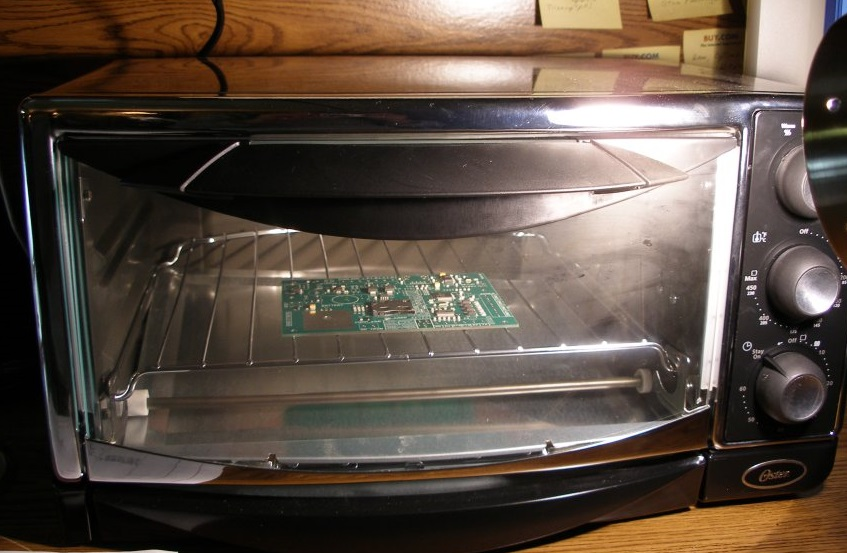
\includegraphics[width=40mm]{resources/boardintheoven.jpg}
	\captionof{figure}{SMD board being reflowed in a toasted oven.}
	\label{toasteroven}
\end{minipage}%
\hfill
\begin{minipage}{.3\textwidth}
	\centering
	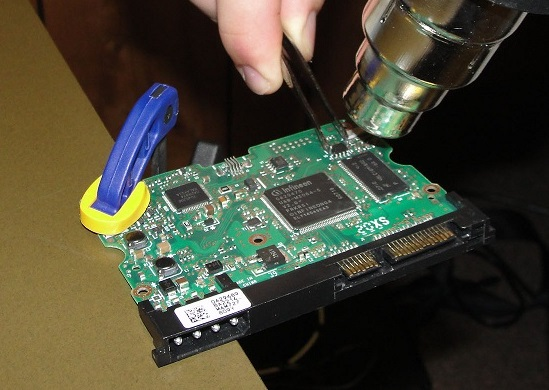
\includegraphics[width=40mm]{resources/hotair_demo.jpg}
	\captionof{figure}{SMD component being soldered with a hand-held hot air gun.}
	\label{hotairdemo}
\end{minipage}%
\hfill
\begin{minipage}{.3\textwidth}
	\centering
	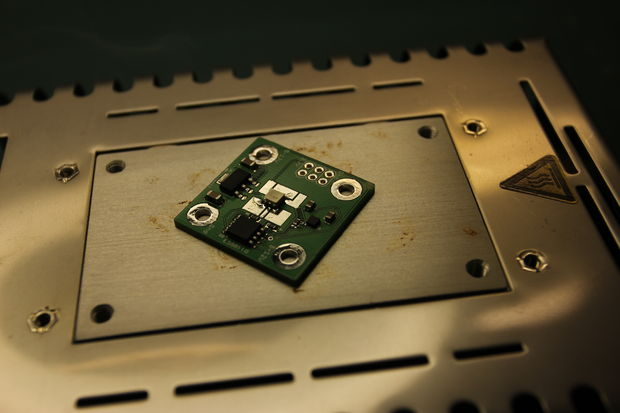
\includegraphics[width=40mm]{resources/hotplate.jpg}
	\captionof{figure}{SMD board being soldered with a hotplate.}
	\label{hotplate}
\end{minipage}
\end{figure}	
			
The choice of method to heat the solder paste may well depend on the end-user - one solution is not clearly superior to the others. During the
course of this project the hand-held hot air gun will be used most often due to equipment availability.

\subsection{Electronics/Firmware}
An AVR chip will be used to translate GCODE to stepper motor commands for the following reasons:

\begin{itemize} \itemsep0em
	\item	Cost: an atmega328 is \pounds 2-3, a USB-serial chip is < \pounds 2, which is not much.
	\item	Mature open source firmware (GRBL, https://github.com/grbl/grbl) is available for GCODE-\textgreater stepper
		conversion, which leaves more time to focus on other parts of this project.
\end{itemize}

On the host pc, custom software will have to be written to translate the design into a GCODE file to be sent to the machine. Usefully however,
the machine's firmware will not need to be written or modified significantly.

\section{Improved designs}

\subsection{Solder paste extruder}

The solder paste extruder design that was initially used was unnecessarily bulky and complex. This made it both harder to fit to the tool mounting mechanism, and increased the
distance between the mount and the tool, amplifying any wobble in the mount. It was therefore deemed necessary to redesign it, optimising for size. Operation and performance
is similar between all designs however.

\subsubsection{Paste extruder using bevel gears}
\begin{figure}[ht!]
\centering
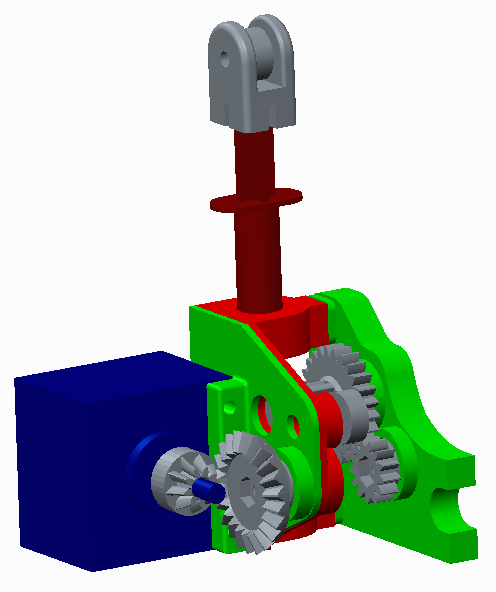
\includegraphics[width=90mm]{resources/extruder_bevel.png}
\caption{Placeholder image of bevel extruder}
\label{overflow}
\end{figure}

The first attempt to reduce the size of the extruder used bevel gears to shrink the size of the gearbox. 

\subsubsection{Paste extruder using worm gears}
\begin{figure}[ht!]
\centering
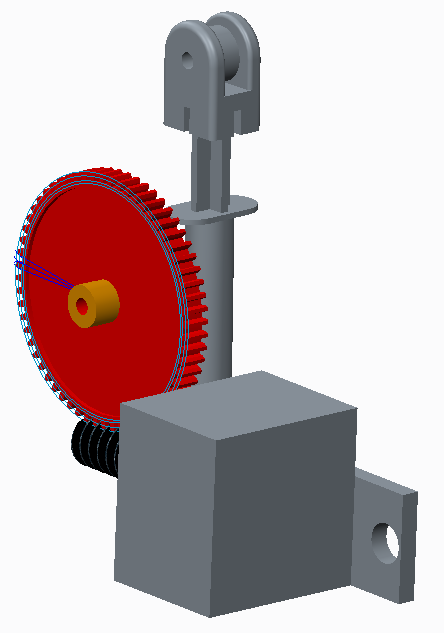
\includegraphics[width=90mm]{resources/extruder_worm.png}
\caption{Placeholder image of worm extruder}
\label{overflow}
\end{figure}

Worm gears would give the same gear ratio in a smaller gearbox, so a new design was made using them. The improved design is as small as possible and performs as well as the much larger extruder that
was originally used.

\section{Serial interface}
For simplicity, the communication between the PC and the electronics board is implemented as a serial link. An arbitrary baud rate of 57600 has been
chosen, this is sufficiently fast so that the electronics board is not slowed by waiting for instructions (as the firmware buffers incoming commands in
a small buffer in RAM), and sufficiently slow that the error rate is assumed to be zero.

\subsection{USB-serial cable}
A USBserial cable based on the FTDI FT232R chipset can be plugged into the serial header on the electronics board. This is a cheap (<\pounds 5) device that is 
a complete solution. Driver support for the FT232R is available for all platforms that have been considered (Windows/OS X/Linux/Android).

%\subsection{Bluetooth serial link}
%\begin{figure}[ht!]
%\centering
%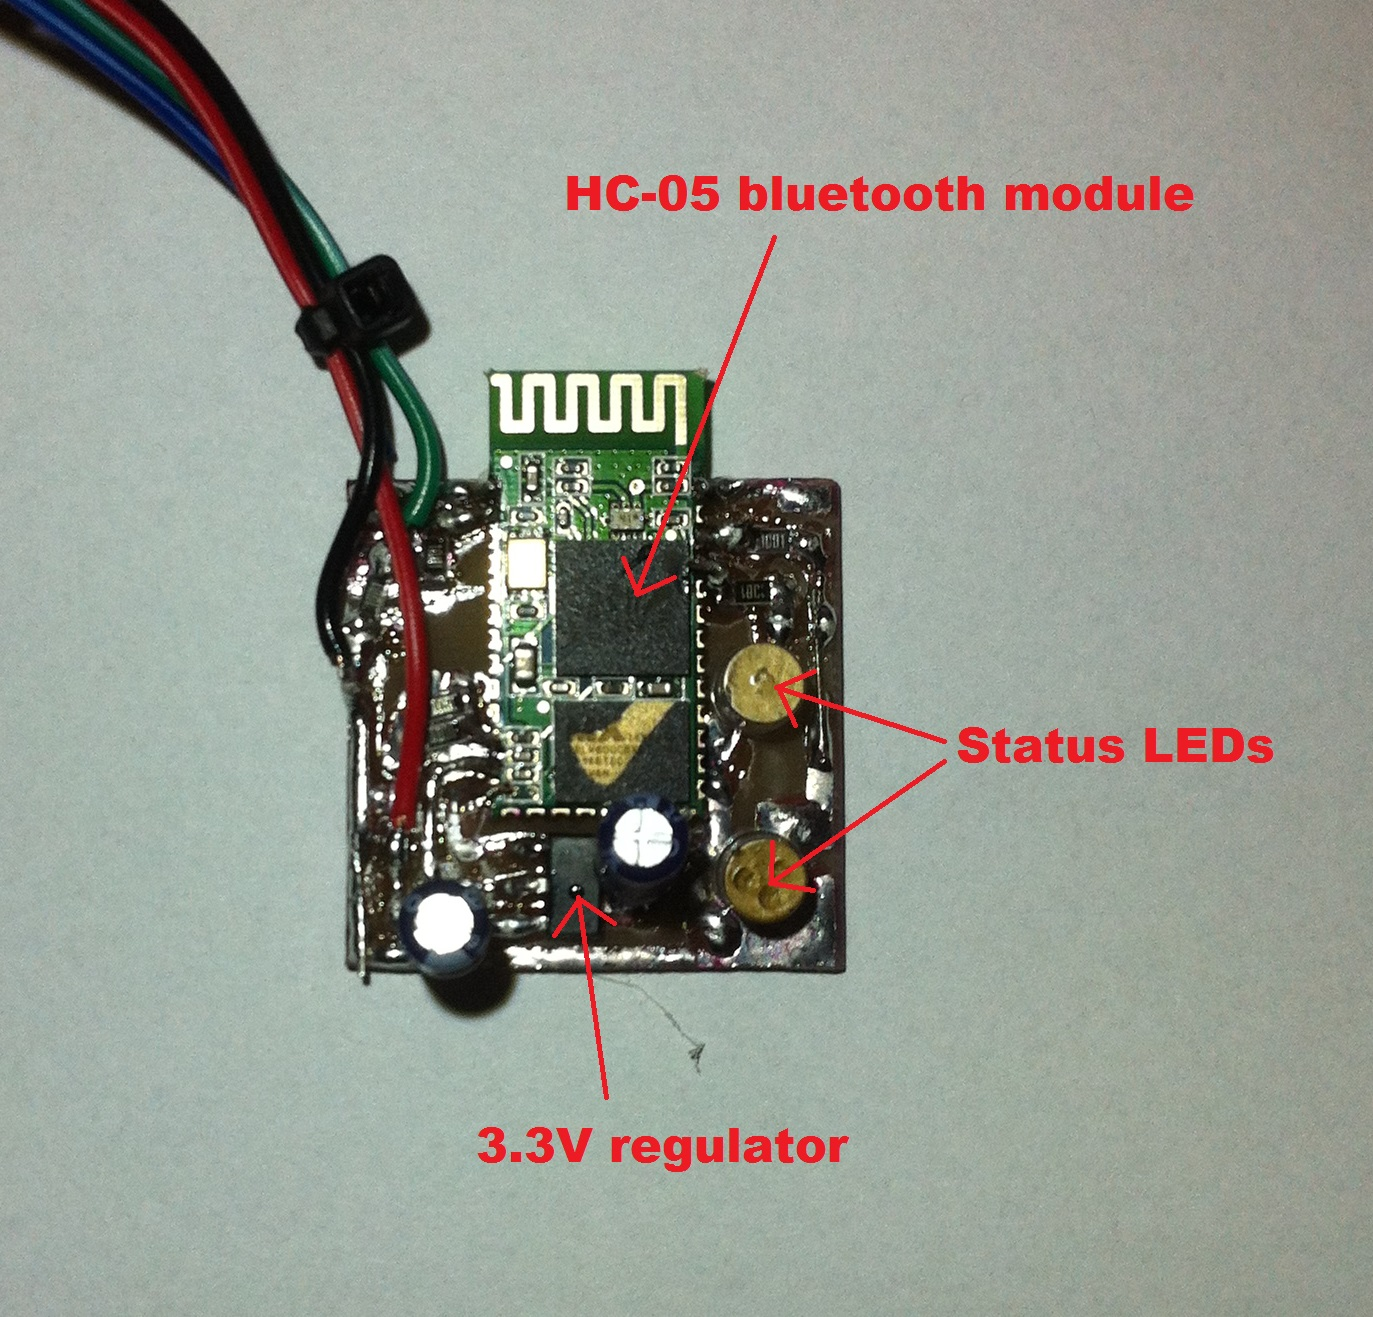
\includegraphics[width=90mm]{resources/bluetoothmodule.jpg}
%\caption{Bluetooth module mounted on breakout board.}
%\label{overflow}
%\end{figure}

%\begin{figure}[ht!]
%\centering
%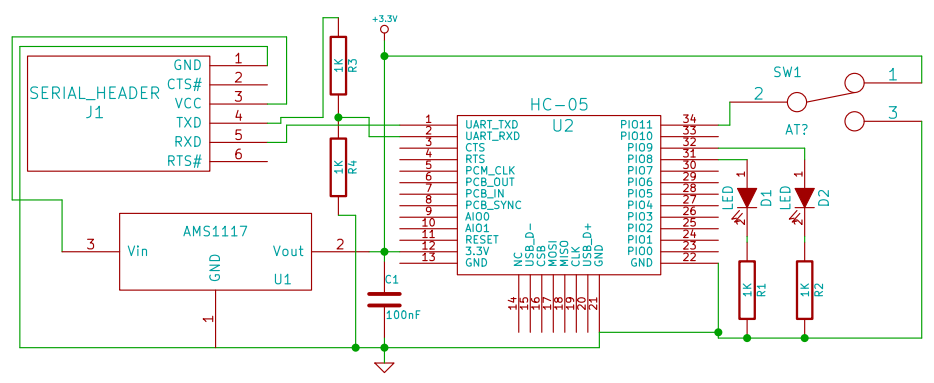
\includegraphics[width=160mm]{resources/hc05breakout.png}
%\caption{Bluetooth breakout module schematic.}
%\label{overflow}
%\end{figure}

As an alternative to a USB-serial cable, a bluetooth link can be used. Depending on the end user, this may be more convenient. The HC-05 bluetooth module was
chosen because of its low cost (\pounds 3.50) and simplicity. The board requires a 3.3V supply, which is not present on the electronics board. A small
breakout board was manufactured for the module, including an AMS1117-3.3 3.3V linear regulator (\pounds 0.10) and link status LEDs. The 3.3V TX output from the module is sufficient
for the AVR despite its higher 5V supply. To avoid damage to the bluetooth module, a potential divider consisting of two 1k resistors is used. This 2.5V output is
again sufficient for the bluetooth module.

To configure the baud rate for the bluetooth module, it was connected to a pc using a USB-serial cable. The bluetooth module is powered up whilst the "KEY" pin is held high (3.3V).
This starts the module in AT configuration mode. The baud rate was then set by sending the string "AT+UART=57600,1,0" at 38400 baud. This configuration is only required once,
the module stores all configuration in non-volatile storage.

\section{Power Supply}
The machine is powered with a 12V 30A power supply. It has over-current and overheating protection built in, but as a failsafe, a 20A fuse is added inline with the +12V cable. 

\section{Host computer software}
Software will have to be written to translate board cad data to gcode. Some of this already exists in the public domain, some will have to be made
as part of this project.

Isolation milling and drilling: pcb2gcode (https://github.com/festlv/pcb2gcode-metric). Takes gerber designs and generates isolation routing/drilling
GCODE. It is also capable of voronai isolation (functionally equivalent routing that cuts the least amount of material). The only configuration
will be to generate a millproject file with the correct cutting depths.

Solder paste placement: No freely available software.

Device placement: No freely available software.

The solder paste placement should be relatively straightforward. The program will simply need to find the locations of the pads, calculate their
area, and then apply a suitable amount of paste to them. For ICs, the paste will not need to be separately applied to each pin (due to the high
surface tension of molten solder), so some method of detecting ICs on the board layout will be needed.

The code to place devices will be the most challenging. However, provided there is a sensible area in which to hand-deposit the devices, it should
not be too hard to calculate how to transport them to the required location.

In my opinion, the most challenging part of writing the conversion code will simply be to extract the necessary data from the cad files. Once this
has been obtained, the GCODE should be easy to create.

\subsection{Improvements to pcb2gcode}
pcb2gcode was forked on github, and the improvements from this project are available at \cite{github}.
To demonstrate the effects of the improvements, pictures of a SOIC-20 breakout board being processed are included (Figures ~\ref{pcb2gcodeinput} , ~\ref{pcb2gcodeisolation} , ~\ref{pcb2gcodepaste} ).

\begin{figure}[ht!]
\centering
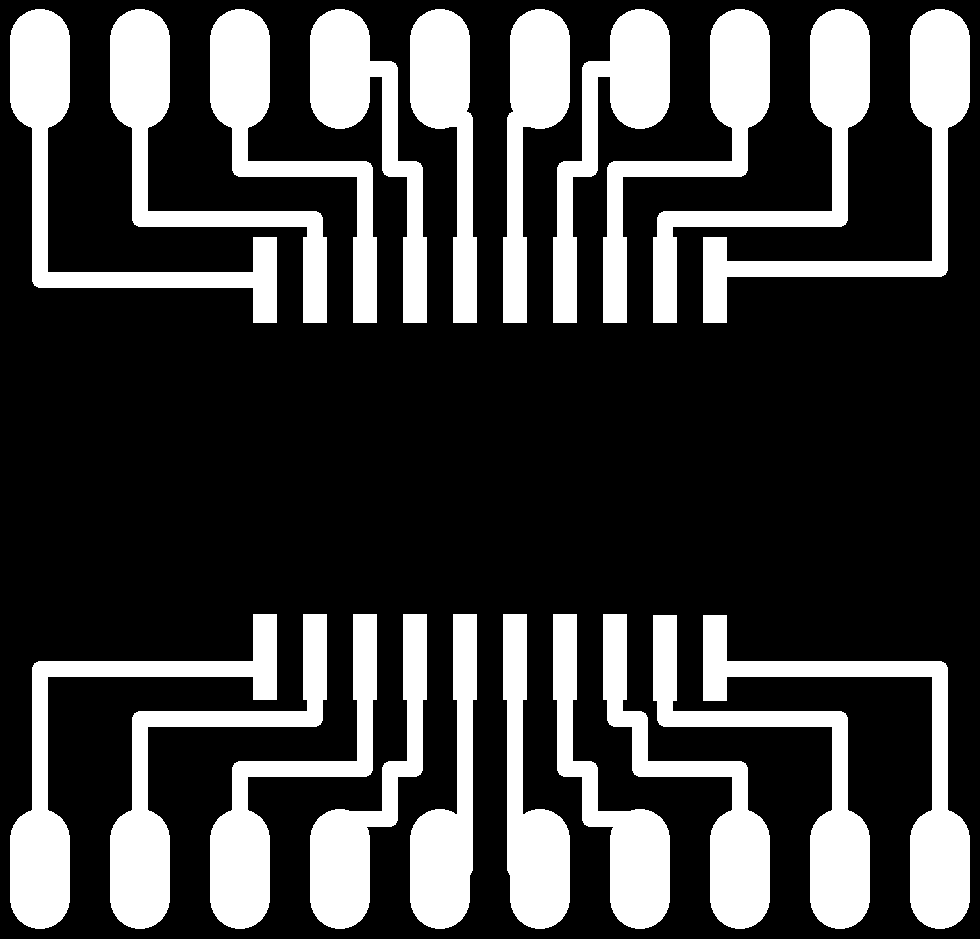
\includegraphics[width=90mm]{resources/breakout_copper.png}
\caption{Input to pcb2gcode, showing the copper traces in white.}
\label{pcb2gcodeinput}
\end{figure}

\begin{figure}[ht!]
\centering

\includegraphics[width=90mm]{resources/breakout_isolation.png}
\caption{Output from pcb2gcode, showing isolation routing pattern (milling to be run between coloured sections).}
\label{pcb2gcodeisolation}
\end{figure}

\begin{figure}[ht!]
\centering

\includegraphics[width=90mm]{resources/breakout_paste.png}
\caption{Solder paste output from pcb2gcode, showing where paste is to be deposited.}
\label{pcb2gcodepaste}
\end{figure}

\subsubsection{Adding solder paste support}
Solder paste information is contained in the GTP (Gerber top paste) file. It was decided to extend pcb2gcode to read this file, and output GCODE suitable for solder paste extrusion.

The GTP file is in the same RS-274X extended Gerber format as the other files that pcb2gcode can already read. For simplicity, the existing Gerber processing was used.
This is retrieved in \begin{verbatim}NGC_Exporter::export_layer(see ngc_exporter.cpp)\end{verbatim}. The data is stored as a vector of vertices of each pad to be filled with solder paste.

An assumption is currently made that all pads are rectangular, and that the paste can be suitably applied in a single place. This may need to be improved in the future if large areas
of solder paste are required.

Process of determining where to deposit paste:

\begin{enumerate}
	\item	Vertices of pad stored in array.
	\item	Area of pad calculated.
	\item	Center of pad calculated.
	\item	From the area of the pad, the diameter of the needle, and the required paste thickness, the extrusion distance is calculated.
	\item	GCODE is written to extrude paste at the center of the pad.
\end{enumerate}

Retraction:

The belt on the paste extruder is slightly springy. This results in the extruder continuing to extrude a small amount of solder paste after the motor has stopped moving.
This has an adverse effect on board quality. To counter this, the extruder should be retracted slightly to remove all pressure from the syringe. The distance to retract
as well as speed of retraction should be experimentally determined for optimum results. Retraction support has been added to the solder paste output of pcb2gcode.

\section{Tools}
In the course of this project, access to a small mill, a 3d printer and a lathe was essential. It may be worth considering that a lot of people/schools have
access to a laser cutter and perhaps mill/lathe, so if possible all custom components could be 3d printed or 
laser cut.

\section{Solder paste extrusion}
Initially, a freely available design for the paste extruder was used \cite{thingipaste}.

The extruder works by applying pressure to the top of the solder paste syringe. Pressure is applied by tightening a pulley made
of T5 timing belt with a geared stepper motor. This design was chosen because the extruder is compact, and the design allows for
fast reduction of pressure, important for clean extrusion and to avoid the solder paste dribbling. 

To calibrate the extruder, two parameters are needed: steps/volume extruded and retraction steps. The first is easy to calculate:

(All dimensions in mm,mm\textsuperscript{2},mm\textsuperscript{3})

The solder paste is supplied in a 2.5ml syringe, with a 66.1276mm\textsuperscript{2} cross-sectional area.

\begin{eqnarray}
\text{Volume extruded / step} &=& \frac{\text{cross-sectional area of syringe} \times \text{T5 pitch} \times \text{number of teeth of T5 pulley}}{\text{number of microsteps} \times \text{steps/revolution} \times \text{gear reduction ratio}} \nonumber \\
&=&\frac{66.1276 \times 5 \times 10}{16 \times 200 \times 12} \nonumber \\
&=&0.0861mm\textsuperscript{3} \nonumber \\
	\text{Steps / mm\textsuperscript{3}} &=& \frac{1} {\text{volume extruded / step}} \nonumber \\
	&=& \frac{1}{ 0.0861} \nonumber \\
	&=& 11.61 \nonumber
\end{eqnarray}

The retraction steps must be experimentally determined. The choice is a trade-off between minimising solder paste dribble (large number
of retraction steps) and reducing total process time (small number of retraction steps). It must be enough that negligible pressure is
exerted on the syringe when retracted.

Some method to "prime" the extruder will be needed. Assuming the extruder is initially hand-tightened so that the belt has little slack,
a possible method is to repeatedly advance the extruder and then retract by a slightly smaller amount, until the user notifies the machine
that solder paste has been extruded. At this point, the extruder should pause after retracting. The solder paste deposition process can
then commence since the exact point of extrusion has been established. 
%Assuming that x is the required granularity of calibration (the 
%maximum amount of solder paste that will be wasted), and y is the retraction distance, the following example GCODE will carry out this calibration:

%\begin{lstlisting}[frame=single]
%//values in braces {} are to be evaluated on the host
%
%//Start loop here:
%G92 E{y} //Set extruder position in firmware to be y
%G1 E{x+y} //Extrude x amount of paste
%G1 E{y} //Retract
%//if user has not indicated extrusion then loop again
%
%//when the user has indicated extrusion:
%G92 E{y}
%\end{lstlisting}
	  
\section{Managing devices prior to placement}
There will need to be a way to place the devices in a known position, so they can then be picked up and placed in their final locations.
Commercial pick and place machines take the parts directly from the reels they are supplied in. While this is optimal for that application in that
it is a very fast way to operate, the cost of reel dispensers is prohibitive for this machine. Instead, the parts will have to be roughly placed
by hand. There are a number of ways this could be done:

\begin{itemize} \itemsep0em
	\item	Embossed outlines of all necessary device footprints.
	\item	Rectangular embossed outline, devices to be located in one corner.
\end{itemize}

It was decided that the latter would be simplest to implement. A rectangular hole will be milled into the bed. Each part can then
be manually placed inside, then pushed to one corner. A consistent system will be needed to ensure correct orientation. The following set of rules
is to be used:

\begin{itemize} \itemsep0em
	\item	ICs will be placed with pin 1 touching the datum corner.
	\item	Devices will always be placed with the longest side (if applicable) touching the long side of the rectangle.
	\item	Devices such as MOSFETs will be placed with the corner between the longest side and side with most pins touching the datum corner.
	\item	Polar 2-lead devices with always have the anode nearest the datum corner.
\end{itemize}

Given the current component to be placed, and the device footprint, it will be trivial to find the coordinates of the centre of the part. Some
consideration will have to be given as to how to determine the centre of mass of parts which are not symmetrical in two directions (e.g. MOSFETs).
	   
\section{Vacuum Placing}
\subsection{Prototype}
To test how effectively small parts could be placed with a vacuum, a simple test setup was fabricated:

\begin{itemize} \itemsep0em
	\item	12V diaphragm air pump (\pounds 8.89 - eBay)
	\item	6mm OD/4mm ID silicone tube (\pounds 2.69/m - eBay)
	\item	various needles (need more info here)
	\item	MOSFET
	\item	330$\Omega$ resistor
\end{itemize}

\begin{figure}[ht!]
\centering
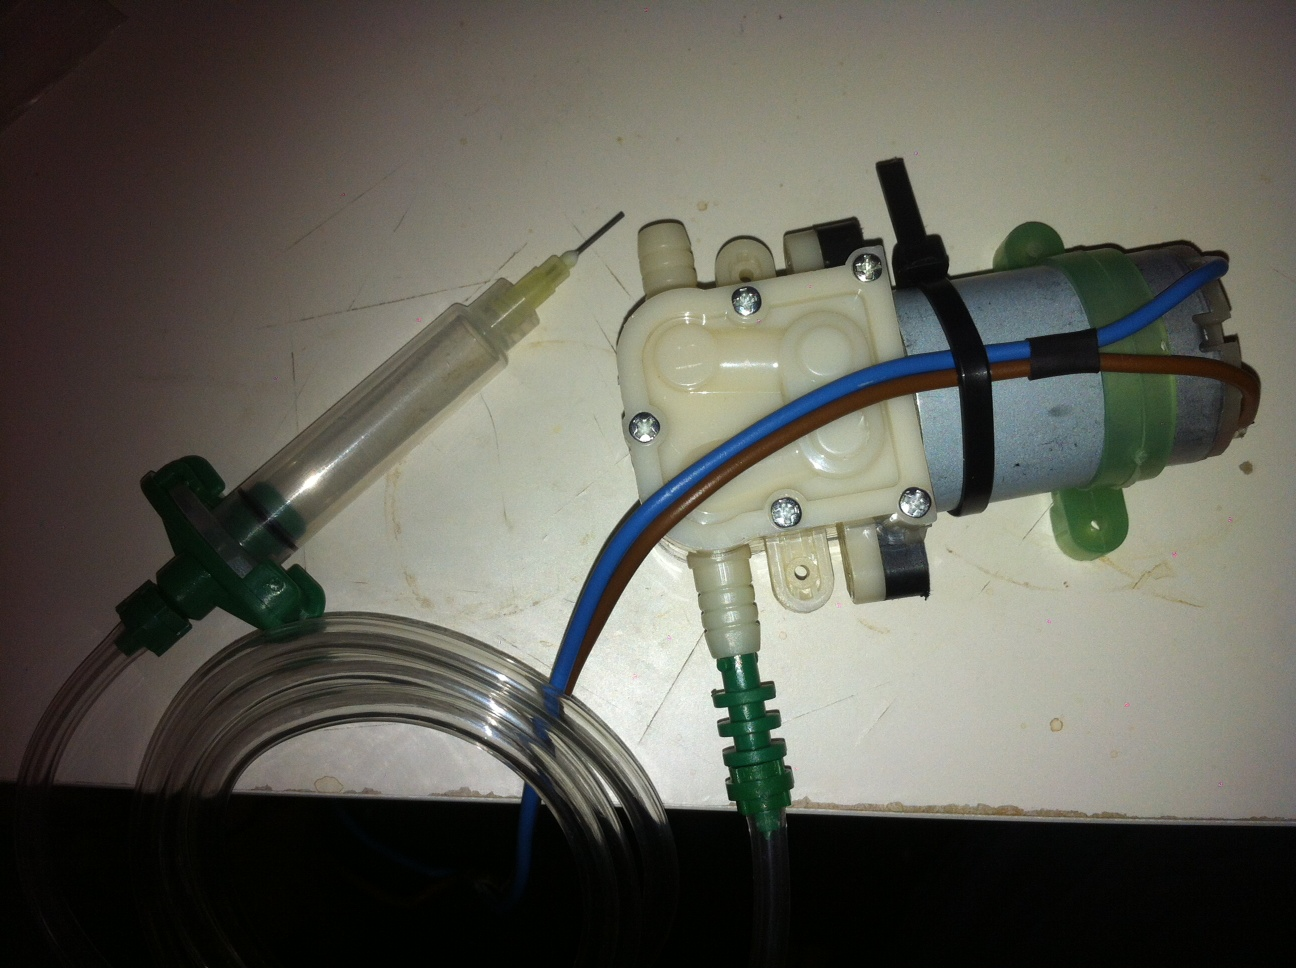
\includegraphics[width=90mm]{resources/pump_and_hose.jpg}
\caption{Pump with hose and needle.}
\label{hose and needle}
\end{figure}

The pump draws ~200mA at 12V, which is easily controlled with a MOSFET. Using a 1.8mm ID needle, SOIC-20 parts were picked up, 
and had significant friction against the needle - essential to avoid slipping or rotating. It was important to place the needle 
as centrally as possible on the part to avoid generating any imbalance that allowed the part to fall. 

\subsection{Conclusions}
A vacuum needle solution is workable, and a good choice for this project. Things that need to be considered for use in the final project:

\begin{itemize}
	\item	The pump takes a certain time to generate a vacuum because of the relatively large internal volume of the pump
		and silicon tube. It will be important to measure this, and add a margin of error so that full suction is applied
		to each device before any movement takes place. Similarly, when turning off the pump, the pressure must return to
		atmospheric before the device can be considered to have been placed successfully. In testing, the pump took
		less than a second to leak sufficiently for this to occur, but if another pump were to be used, it may be necessary
		to place a tiny hole in the air line so that pressure drops quickly.
	\item	It is important to place the needle very near to the centre of mass of the device. The majority of devices will be
		symmetrical, which will make this easier.
	\item	The needle must be able to be raised and lowered to the correct heights. It may be possible to push the needle down
		with a weak spring, with a micro servo that raises it - this would remove any need to know the exact height of each
		device. This will need to be tested.
\end{itemize}

\begin{figure}[ht!]
\centering
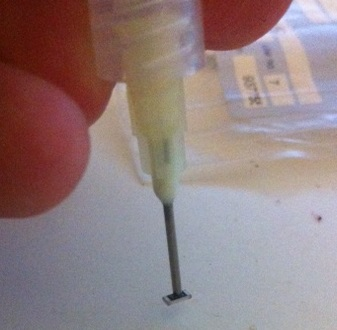
\includegraphics[width=90mm]{resources/needle_with_resistor.jpg}
\caption{SMD resistor being picked up.}
\label{overflow}
\end{figure}

\section{Operating Speed}
For the machine to be practical, there are some limitations on the maximum time that a board can take to manufacture. This is particularly true of the device placement stage, as this requires
human intervention. The total time can be divided into a few main sections:

\begin{itemize}
	\item	X/Y travel.
	\item	X/Y cutting.
	\item	Z movement.
	\item	Picking/placing components.
	\item	Hot air reflow.
\end{itemize}

The X/Y travel will take the most time in total, so the estimated times should be calculated and optimised if possible. Assuming a travel speed of 10mm/s, the total
time is simply total distance (mm) / 10.

\section{Measuring Accuracy}
\begin{figure}[ht!]
\centering
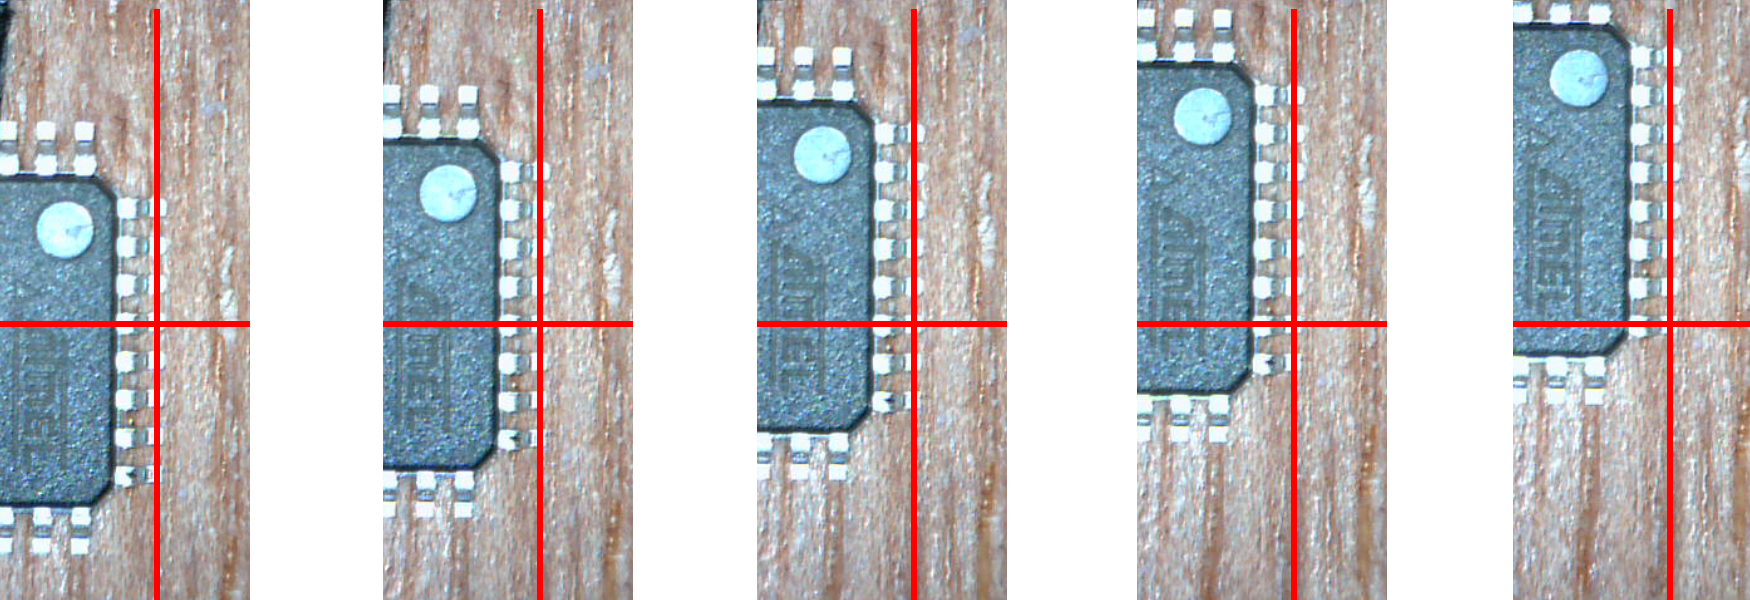
\includegraphics[width=170mm]{resources/registration.png}
\caption{Visual alignment test using one side of a TQFP-32 Atmega328.}
\label{overflow}
\end{figure}

It is important to measure the accuracy of the axes to ensure that they can reach the specified +-0.05mm. This will need to be measured
at all points on the bed (as the accuracy will worsen when the bed is central due to increased rod deflection.). Of particular concern will be
the deflection under the load of the isolation routing bit. The solder paste and device placement will not involve any significant force. The 
drilling will generate a force, but the tolerance required of a 1mm hole is not nearly as demanding as that of the isolation routing cutter.
The exact forces exerted by the routing bit have yet to be measured, but are estimated to be 5-10N. This means that the anti-backlash nut
will need to exert the same or greater force to ensure that the board does not move. This in turn places extra resistance on the motor movement.

\subsection{Testing methodology}

\begin{figure}[ht!]
\centering
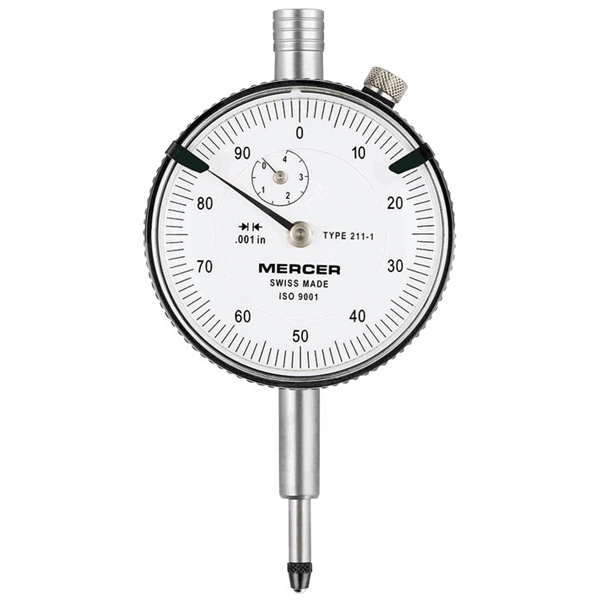
\includegraphics[width=90mm]{resources/dialgauge.png}
\caption{Measurement setup (This is a placeholder image).}
\label{dialgauge}
\end{figure}

In order to characterise the accuracy of the machine, it is important to have a consistent measuring regime. A dial gauge is used to measure
relative positions of the axes. See Figure ~\ref{dialgauge} for the experimental setup. It is important to ensure the worst-case error is acceptable. The causes of error and their effects are:

\begin{figure}[ht!]
\centering
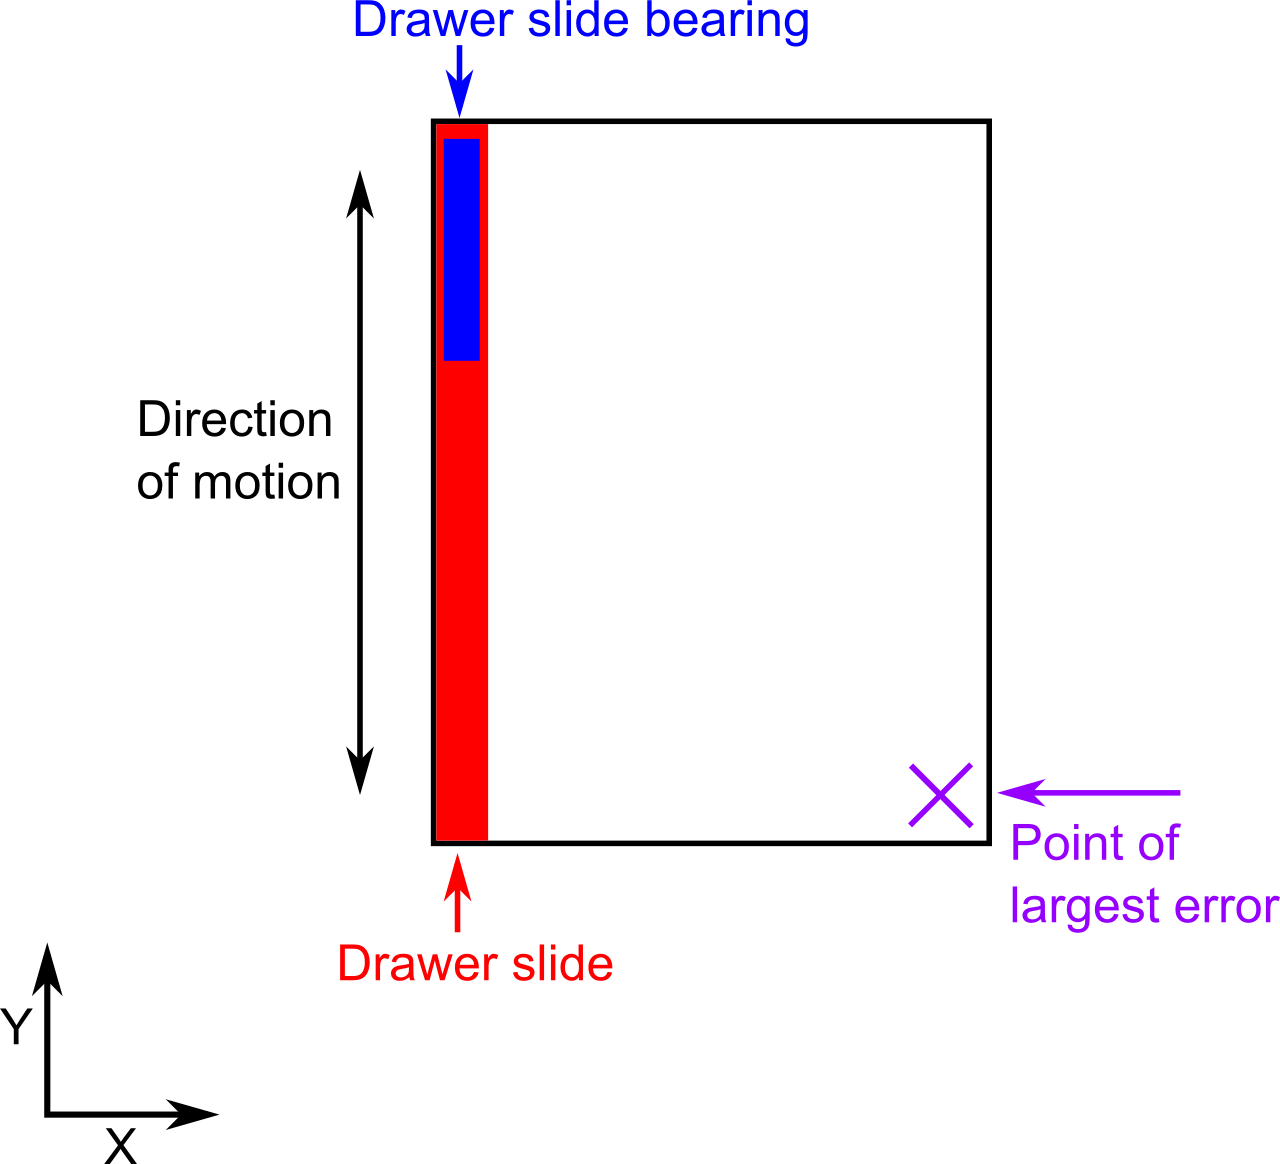
\includegraphics[width=150mm]{resources/errors.png}
\caption{Measurement setup, showing error notation.}
\label{errornotation}
\end{figure}

Effects are shown with reference to Figure ~\ref{errornotation}, noting that the X and Y referred to in the figure do not necessarily represent the machine axes.
\begin{itemize} \itemsep0em
	\item	Z displacement: It is possible the surface of the bed will move in the vertical direction, something that should not happen ideally. This 
			will occur if the surface over which the idler bearing runs is not flat, or due to manufacturing tolerances in the linear slides.
	\item	Rotation: The drawer slides do not eliminate rotation completely, and this error dominates. Rotation is relative to the small ball bearing array which slides along
			the drawer slides, so this source of error depends on the absolute slide position. Figure ~\ref{errornotation} shows the largest error possible, with the ball bearings
			far away from the location of maximum error, where rotation effects dominate.
	\item	Motion parallel to the axis direction. This error is mostly caused by flex in the stepper motor mounts, the motor-\textgreater threaded rod couplers and the anti-backlash nuts.
	\item	Motion perpendicular to the axis direction. This error is caused by small amounts of slop in the drawer slides.
\end{itemize}

As it is only important to measure the worst-case error, the point shown in purple in Figure ~\ref(errornotation) is the only point which will be measured. 

\section{Hot air tool}

\begin{figure}[ht!]
\centering
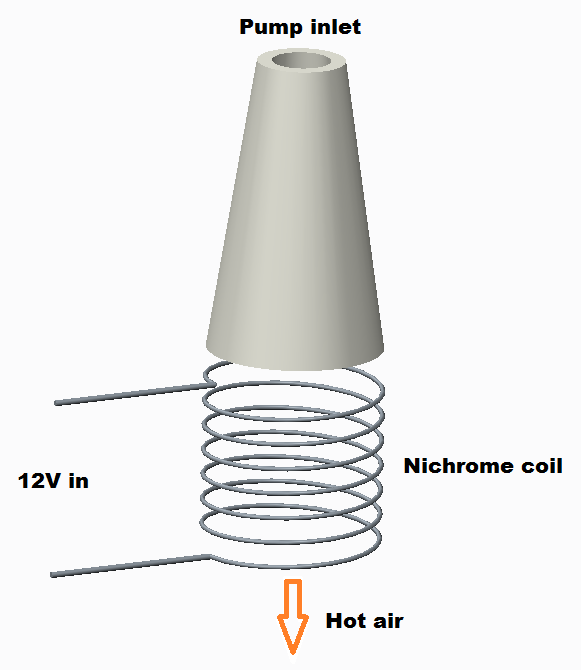
\includegraphics[width=90mm]{resources/hotair.png}
\caption{Simplified diagram of hot air tool.}
\label{overflow}
\end{figure}

Ideally the heating of the solder paste should be carried out automatically by the machine. This section describes a prototype hot air tool.

A hot air tool used for soldering has the following requirements:

\begin{itemize} \itemsep0em
	\item	Ability to heat solder paste up to $240\,^{\circ}\mathrm{C}$
	\item	Slow, steady airflow
	\item	Controllable temperature (i.e. not open-loop)
\end{itemize}

\subsection{Calculations}

Assumptions:
\begin{itemize} \itemsep0em
	\item Specific heat capacity of dry air is not significantly affected by temperature for estimates of power required.
	\item 50\% of energy into heater is used to heat hot air stream (other radiative losses)
	\item Flow rate of air pump = 18 cm\textsuperscript{3} / s
	\item Specific heat capacity of dry air = 1.006 J/gK. This is assumed to not change significantly with temperature (acceptable to $\pm$ 10\%).
	\item Room temperature of 20\textsuperscript{0}C, temperature required is 240\textsuperscript{0}C. Delta T = 220K
	\item Density of air = 0.001225 g / cm\textsuperscript{3}
\end{itemize}

Power required to heat air (ideal) = (18*0.001225)*220*1.006 = 4.88W
Power required to heat air (assuming losses) = 4.88*2 = 9.76W

For simplicity, it is assumed that the heater requires 10W of input power.

The design is based on a small coil of nichrome resistance wire as a heating element. Calculations must be made to find
the size of wire required:

Size of coil (Chosen to be similar in diameter to the air tube with 6mm OD/4mm ID)

Diameter = 5mm
Length = 12mm
Wire spacing = 2mm
Angle of wire = tan\textsuperscript{-1} (2/(5* pi )) = 7.26 \textsuperscript{0}
Turns of wire = 12/2 + 1 = 7
Length of wire = 7 * sqrt ((5 * pi )\textsuperscript{2}  * 2\textsuperscript{2}) =  110.84mm

Resistivity of nichrome at room temperature = 1.0 * 10E-6 ohm m 
Power supply voltage = 12V
Current draw = 10 / 12 = 0.83 A 
Resistance required = 12\textsuperscript{2} / 10 = 14.4 ohms
Cross sectional area of wire = 1.0 * 10\textsuperscript{-6} * 110.84 * 10\textsuperscript{-3} / 14.4 = 7.70 * 10\textsuperscript{-9} m\textsuperscript{2} = 7.70 * 10\textsuperscript{-3} mm\textsuperscript{2}
Diameter of wire = sqrt(7.70E-3/pi) * 2 = 0.099mm

This is the minimum diameter of wire. Next the maximum diameter of wire is calculated, assuming a maximum current draw of 10A.

Resistance required = 12 / 10 = 1.2 ohms
Cross sectional area of wire = 7.70 * 10\textsuperscript{-3} * (14.4/1.2) = 0.092 mm \textsuperscript{2}
Diameter of wire = sqrt(0.092/pi) * 2 = 0.34mm

Therefore wire diameter is between 0.099mm and 0.34mm
The most commonly available suitable wire is sold as 30 SWG, equivalent to 0.315mm diameter.

Resistance of 110.84mm of 0.315mm diameter nichrome wire:

\begin{displaymath}
\text{Resistance} = \frac{\rho L}{A}
= \frac{1.0*10^-6*110.84*10^-3}{\pi*(\frac{0.315*10^-3}{2})^2}
= 1.42 \Omega
\end{displaymath}



\begin{displaymath}
\text{Maximum current draw} = \frac{\text{V}}{\text{R}}
= \frac{12}{1.42}
= 8.45 \text{A}
\end{displaymath}

\section{Standalone Operation}
It may be useful to operate the machine without a connected PC. In the case of manufacturing a large number of boards, it may be impractical to dedicate a PC simply to sending GCODE.
In addition, some functions of the machine produce dust, and are noisy. Allowing the machine to operate in a more remote location could be convenient. 

The steps taken to produce GCODE (e.g. running pcb2gcode) will always need a PC, but once the GCODE has been produced it is possible for the machine to read this from connected storage.

\subsection{SD card reading}
SD cards are ideal for use with microcontrollers, as they have a simple protocol (SPI), and are inexpensive. They also have wide compatibility with other devices. It would be useful if 
the GCODE could be stored on an SD card and read by the machine.

\subsubsection {Hardware}
SD cards can operate in SPI mode, using only four connections (MISO, MOSI, CLK, CS). However, they operate at 3.3V, and the AVR operates at 5V. To power the card, an AMS1117-3.3 linear regulator
is used. Level translation must be used to convert the four connections to the required voltages. There are three options for this process:

\begin{itemize} \itemsep0em
	\item	Potential dividers. This is the simplest option, using only resistors. The CS, MOSI and CLK connections send data to the SD card. A potential divider is used to reduce the voltages
			from 5V to 3.3V. The MISO connection receives data from the SD card. The AVR has a high input threshold of above 2.6V. MISO can therefore be connected as it operates up to 3.3V. 
			Although this is the simplest option, the high impedance output from the potential divider can cause problems at fast SPI speeds, as the SD card presents a relatively high
			capacitive loading.
	\item	Discrete transistors can be used to translate between 3.3V and 5V. This has the advantage of faster operation, and increasing the noise margins (reduced when using 3.3V with a 5V chip).
			Two transistors are needed for each connection to ensure the signal is not inverted.
	\item	A level translation IC can be used. This needs no additional components (except from a decoupling capacitor).
\end{itemize}

\subsubsection {Firmware}
The Marlin firmware used in the machine has full support for SD cards, provided they are formatted with the FAT filesystem.

\subsection{LCD + User interface}
If the machine is to be used in a standalone capacity, there must be a way for the user to choose which GCODE file to send.

\subsubsection{Hardware}
A 4x20 LCD is used to display information about the current job, as well as allow the user to select GCODE files. This is an inexpensive part based on the ubiquitous HD44780 controller chip.
It is operated in 4-bit mode (as opposed to 8-bit mode, which requires four additional microcontroller pins). Six connections are required to the microcontroller: RS, EN, D4, D5, D6, D7. As
the electronics board does not have many spare connections, it was decided to use an MCP23017 i2c port expander to connect the LCD. The Marlin firmware already supports this, and needs just
two connections (SDA and SCL) to the driver board. See Figure ~\ref{lcd_backpack} for the schematic.

\begin{figure}[ht!]
\centering
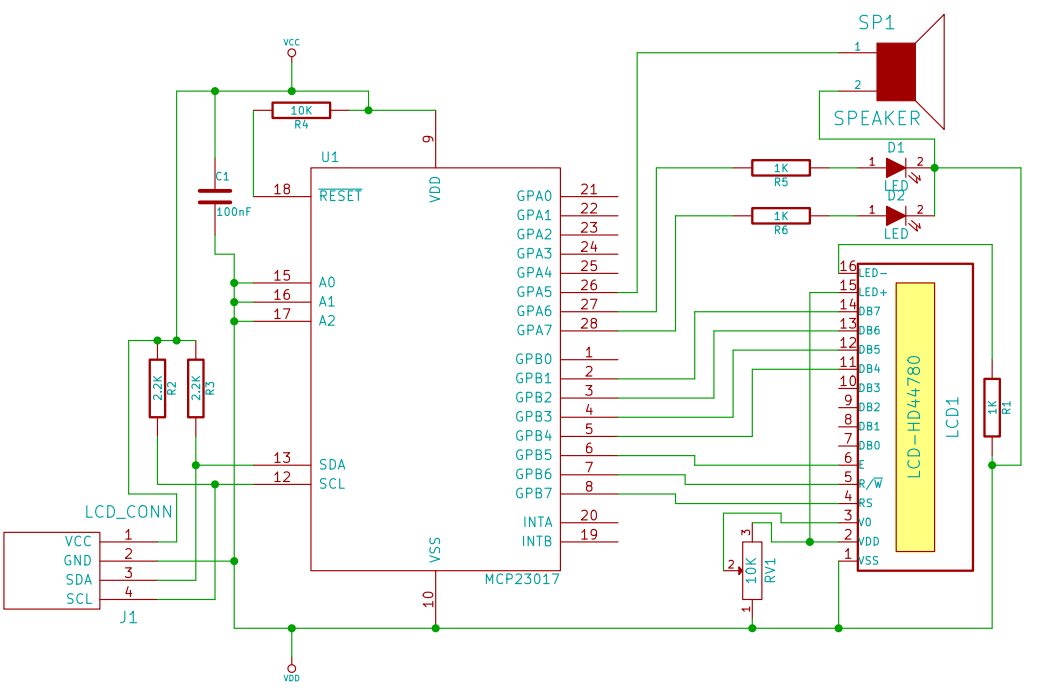
\includegraphics[width=160mm]{resources/lcd_backpack.png}
\caption{Schematic of i2c -> LCD board.}
\label{lcd_backpack}
\end{figure}

A rotary encoder is used to provide input. This uses quadrature outputs to determine motion. The encoder also has a push switch inside for selecting options. This therefore require three microcontroller
pins in total.

\subsubsection{Firmware}
Marlin has support for the LCD and encoder, requiring only a change to Configuration.h and pins.h


\section{Milling}
The spindle on the machine is quite capable of light milling, with some limitations:

\begin{itemize} \itemsep0em
	\item	Milling bits only protrude from the spindle by approximately 8mm (depending on the bit). This means that this is the deepest cut the machine is capable of making.
	\item	The axes do not have the rigidity required for milling tough materials. Plastics and wood are possible, while metals are not.
	\item	The spindle only supports parts with a 3mm shank.
	\item	The spindle speed is variable from 1000-\textgreater40000rpm unloaded. The speed controller attempts to maintain the rotational speed setpoint, however it prioritises
			correct motor commutation. Therefore at higher speeds under heavy loads care must be taken that the spindle speed does not drop significantly. In practice this is unlikely
			to be a problem, as the motor has a maximum power of 250W and has significant moment of inertia.
\end{itemize}

As this functionality is not a central focus of this project, only a simple demonstration of milling ability was done. The spur gear used in the gear extruder is cut from 6mm acrylic:

\subsubsection {Gear CAD}
The gear design was copied into a CamBam project. Ideally the Creo design could have been exported as a .DXF file, but errors were encountered while attempting this. CamBam was used to 
generate GCODE for milling the gear, taking into account the machine's slow travel speeds. The firmware used in the machine does not handle parentheses in the GCODE, so the CamBam 
output must be checked for them, and the lines removed.

\subsubsection {Milling Settings}

The following settings were used to mill the green acrylic gear (Figure ~\ref{fig:gearcomparison}):

\begin{center}
	\begin{tabular}{| l | l | p{8cm} |}
	\hline
	Setting & Value & Comments \\ \hline
	Sheet material & 3mm green acrylic & \\ \hline
	Cutting bit & 1mm diameter endmill & Cambam estimated maximum endmill size to be ~1.4mm diameter. \\ \hline
	%conventional milling
	Depth increment & 1mm & Chosen to produce part quickly at the expense of edge quality. \\ \hline
%	12mm clearance plane
	Cut feedrate & 70mm/min & Very slow feedrate chosen for initial tests. \\ \hline
	Plunge feedrate & 70mm/min & Slow feedrate to avoid chips clogging.\\
	\hline
	\end{tabular}
\end{center}

\subsubsection {Envisioned uses for milling}
{
There are a number of uses for a machine capable of light milling:

\begin{itemize} \itemsep0em
	\item	Manufacturing PCBs with arbitrary shapes. For example, It is possible to build connectors from PCBs that lie on the circuit board if they can be milled to the correct shape.
			For example, USB connectors. This reduces part cost.
	\item	Improving the finish of 3d printed components. In cases where the rough edges of 3d printed parts are not satisfactory, a milling pass over the piece can increase the flatness
			of edges.
	
\end{itemize}
}

\begin{figure}[ht!]
\centering
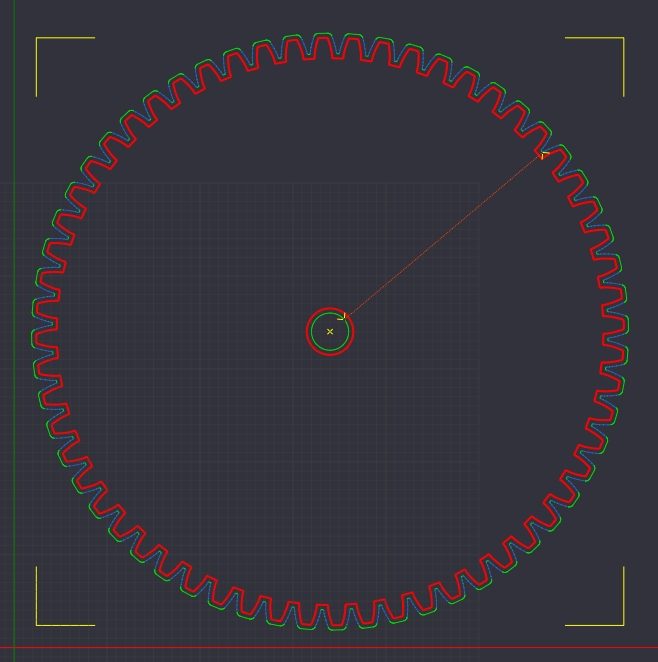
\includegraphics[width=90mm]{resources/gear_cambam.png}
\caption{Gear outline shown in red. Toolpath shown in green/blue.}
\label{overflow}
\end{figure}

\begin{figure}[ht!]
\centering
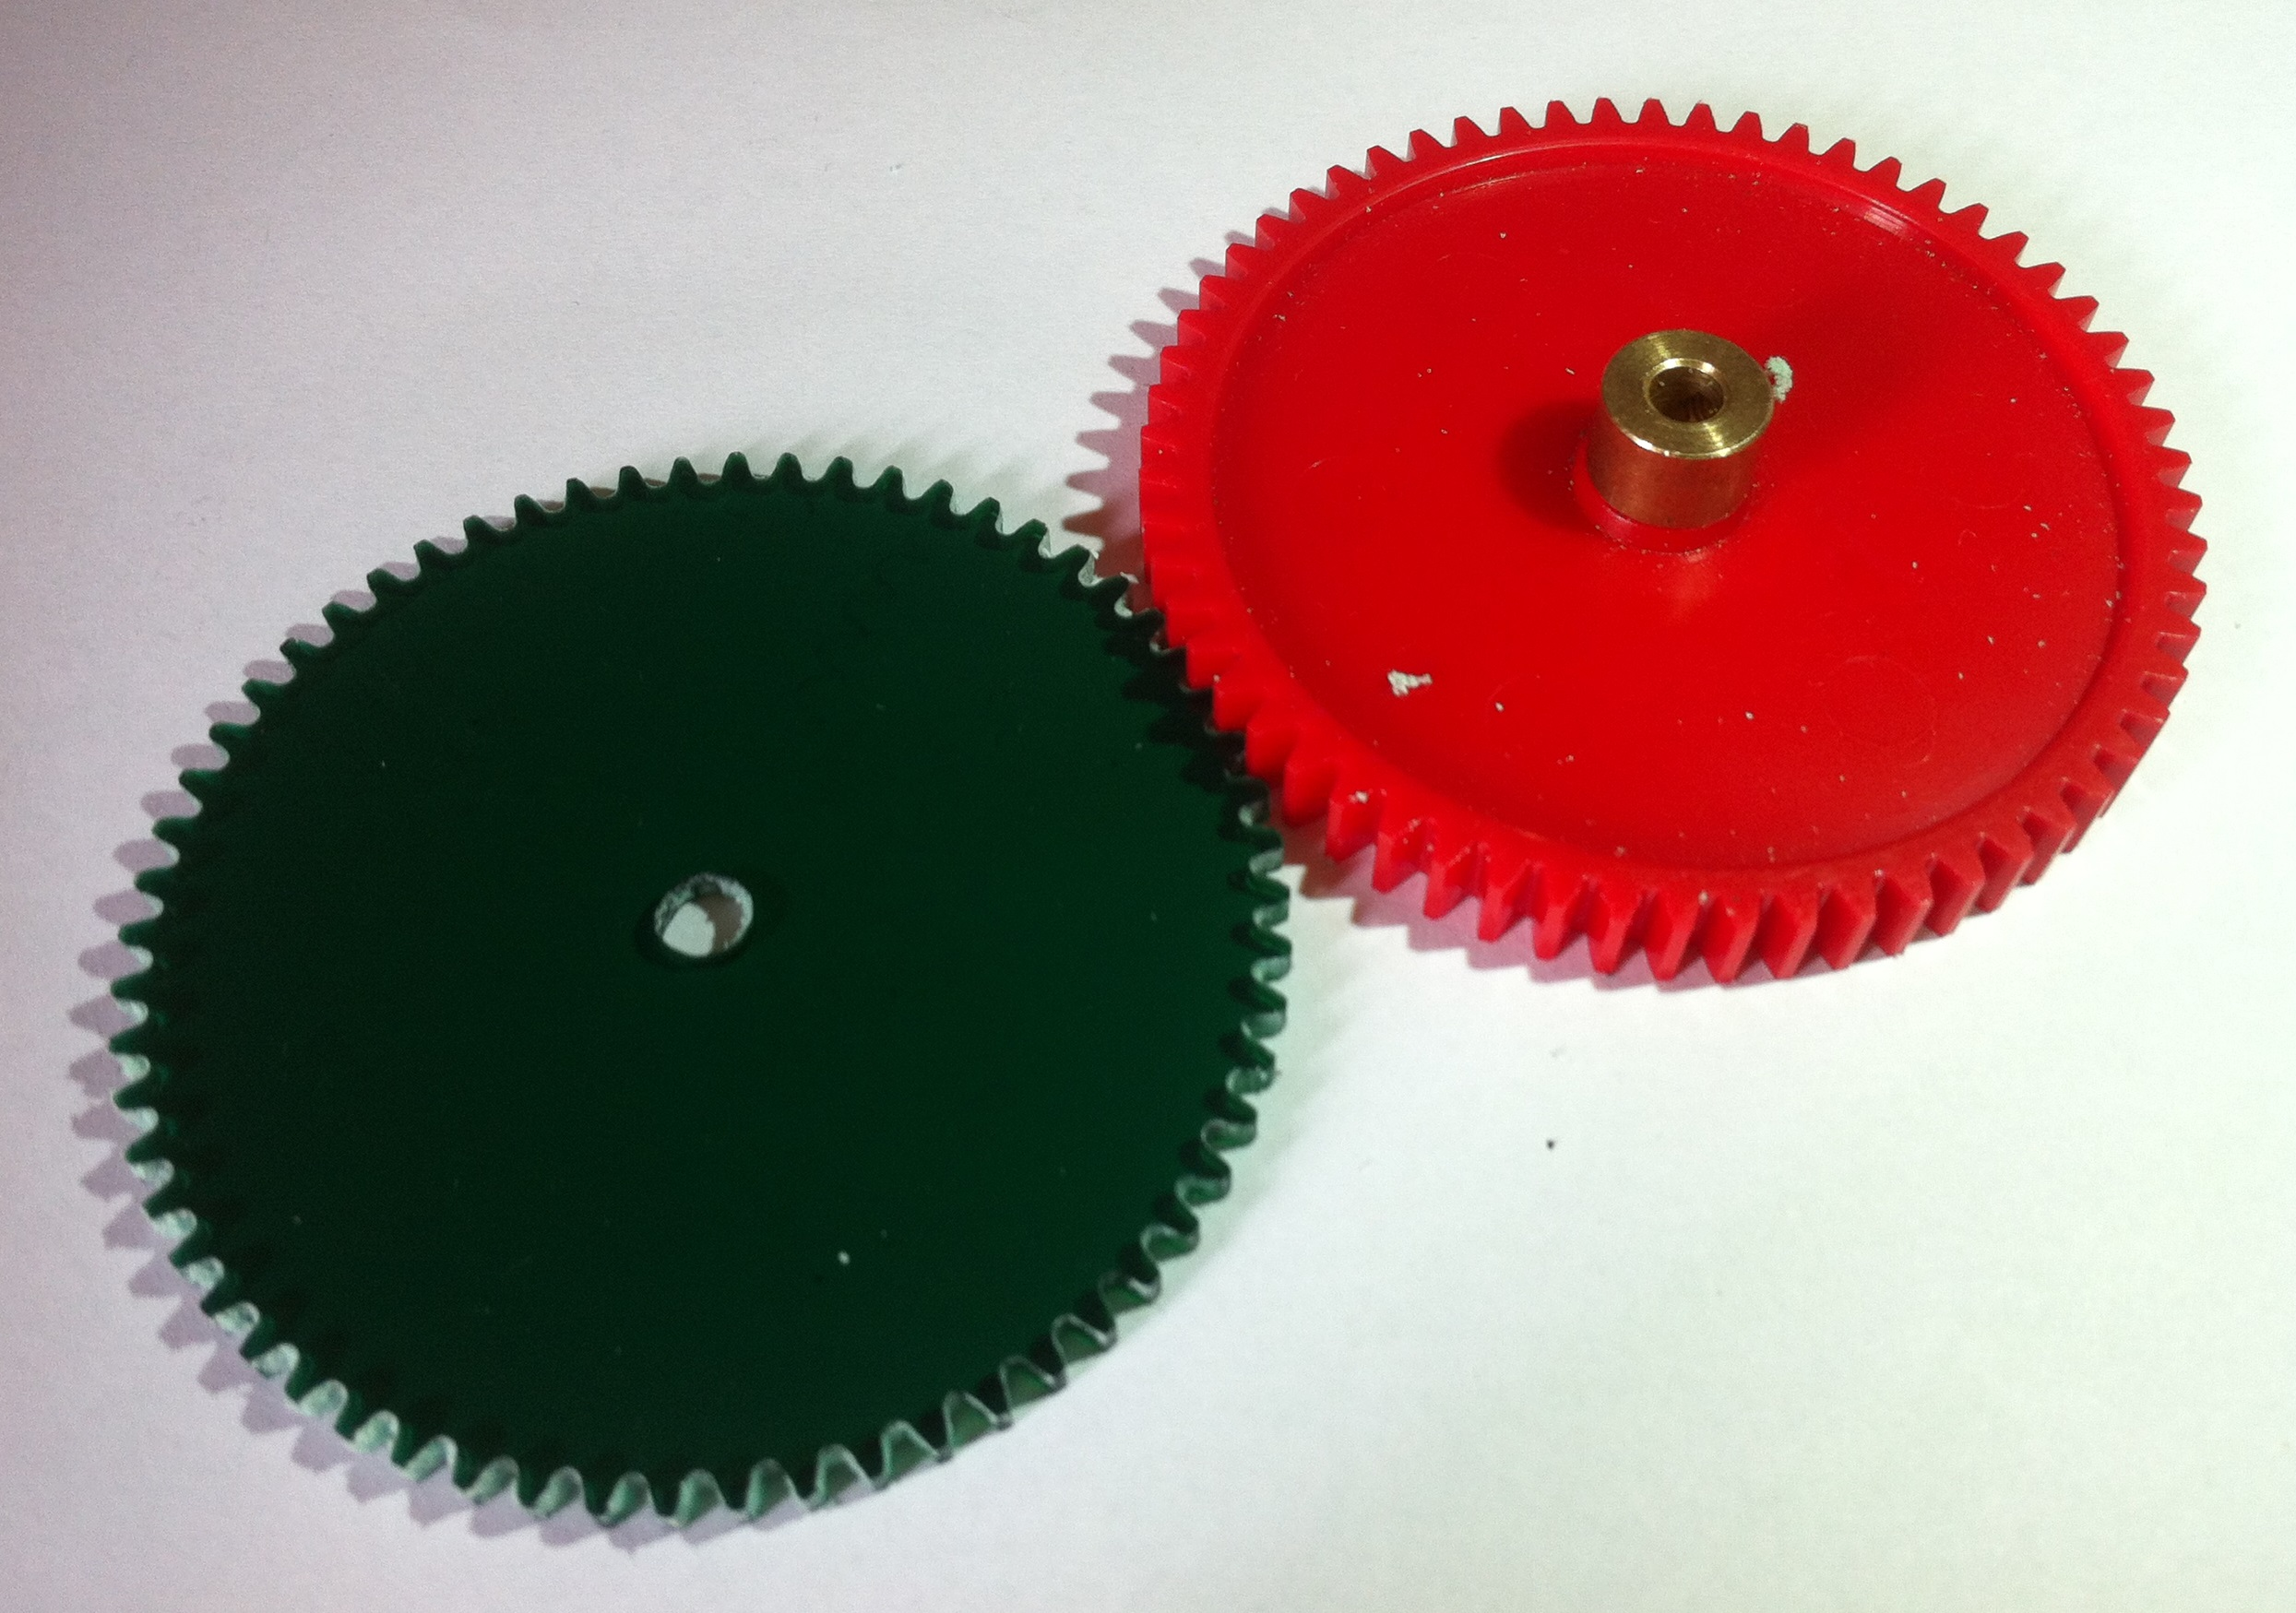
\includegraphics[width=90mm]{resources/gear_comparison.jpg}
\caption{Milled gear (left) compared to original gear (right).}
\label{fig:gearcomparison}
\end{figure}

\section{Operating Steps}

% Define block styles
\tikzstyle{decision} = [diamond, draw, fill=blue!20, 
    text width=4.5em, text badly centered, node distance=3cm, inner sep=0pt]
\tikzstyle{block} = [rectangle, draw, fill=blue!20, 
    text width=14em, text centered, rounded corners, minimum height=3em]
\tikzstyle{line} = [draw, -latex']
\tikzstyle{cloud} = [draw, ellipse,fill=red!20, node distance=7cm,
    minimum height=2em]
    
\begin{tikzpicture}[align=center,node distance = 1.6cm,auto]
    % Place nodes
    \node [block] (pcb2gcode) {run pcb2gcode to generate GCODE};
    \node [cloud, left of=pcb2gcode, align=center] (designfiles) {PCB designs exported\\ from design package\\ in GERBER format};
    
    \node [block, below of=pcb2gcode] (isolationinit) {attach spindle, load isolation milling bit, zero};
    \node [block, below of=isolationinit] (isolation) {send routing GCODE to machine};
    \node [block, below of=isolation, fill=orange!70] (isolationcheck) {visually check board for errors};
    
    \node [block, below of=isolationcheck] (drillinit) {load drill bit, zero};
    \node [block, below of=drillinit] (drill) {send drilling GCODE to machine};
    \node [block, below of=drill, fill=orange!70] (drillcheck) {visually check board for errors};
    
    \node [block, below of=drillcheck] (pasteinit) {load paste extruder};
    \node [block, below of=pasteinit] (paste) {send solder paste GCODE to machine};
    \node [block, below of=paste, fill=orange!70] (pastecheck) {visually check board for errors};
    
    \node [block, below of=pastecheck] (vacuuminit) {load vacuum needle};
    \node [block, below of=vacuuminit] (vacuum) {send pick and place GCODE to machine};
    \node [block, below of=vacuum, fill=orange!70] (vacuumcheck) {visually check board for errors};
    
    \node [block, below of=vacuumcheck] (reflow) {Heat board to melt solder paste};
    % Draw edges
    \path [line,dashed] (designfiles) -- (pcb2gcode);
    \path [line] (pcb2gcode) -- (isolationinit);
    \path [line] (isolationinit) -- (isolation);
    \path [line] (isolation) -- (isolationcheck);
    \path [line] (isolationcheck) -- (drillinit);
    \path [line] (drillinit) -- (drill);
    \path [line] (drill) -- (drillcheck);
    \path [line] (drillcheck) -- (pasteinit);
    \path [line] (pasteinit) -- (paste);
    \path [line] (paste) -- (pastecheck);
    \path [line] (pastecheck) -- (vacuuminit);
    \path [line] (vacuuminit) -- (vacuum);
    \path [line] (vacuum) -- (vacuumcheck);

    \path [line] (vacuumcheck) -- (reflow);
 %   \path [line] (isolation) -- (isolationcheck);
 %   \path [line] (isolationcheck) -- (drillinit);

\end{tikzpicture}

\section{Zeroing the axes}

When the machine is used it is necessary to "zero" the axes to a known datum point on the board. This is particularly important when swapping tools, as there may
be a small amount of slop in the tool mounts which will vary between tools.

\subsection{X and Y axes}

In order to zero the machine in the X and Y directions, an "L-shaped" piece of metal has been added to the bed (insert pictures/diagrams). All of the tools are metal,
and therefore conductive. The axes are first manually moved to be near-zero. The tips of the tools are all electrically connected to an input pin on the AVR, with a weak (10K) pullup to 5V.
The "L-shaped" piece of metal is connected to ground. When instructed, the firmware slowly moves the X or Y axis in the negative direction until a contact is made, and the input goes LOW. At this point,
the exact position of the tool is known. For convenience it is important that the location of the centre of the tool is known, this can simply be calculated as the diameters of all of the tools are known and fixed.

\subsection{Z axis}

Slightly different mechanisms are used for the zeroing of the Z axis when used for different tools:

\subsubsection{Vacuum needle}

A small microswitch is part of the vacuum needle assembly. It is triggered when the needle is touching either the bed or the top of a component. As a result, zeroing can be carried out simply by 
moving the tool downwards until it is triggered.

\subsubsection{All other tools}

The other tools are zeroing electrically using the same mechanism as for the X and Y axes. The tools are lowered until contact is made between the PCB and the tool. A temporary contact must be made from ground
to the copper pcb, this is achieved with an alligator clip.

\section{Future Work}
This section contains envisioned improvements to the machine that were not implemented due to time constraints.

\subsection{Double-sided boards}
It is common to use double sided PCBs in order to achieve more compact circuits. The machine will not currently have the ability to process such boards, although this would be possible in a later version.

\subsubsection{Challenges}
There are a number of challenges associated with working with dual sided boards:

\begin{enumerate}
	\item	Clamping the PCB to the bed of the machine is more complex with the second side of a double sided board. The components that have
			already been populated will not allow the board to sit flat and level.
	\item	The PCB material is a moderately good conductor of heat. When the second side of the board is heated to melt the solder paste, there
			is a danger that components on the bottom will be loosened and fall off.
	\item	Both sides of the board must be precisely aligned so that any through-holes or vias line up.
	\item	Any vias that are required will add considerable complexity. Commercially they are manufactured in a multi-stage chemical process
			which is not feasible for the hobbyist.
\end{enumerate}

\subsubsection{Envisioned solutions}

\begin{enumerate}
	\item	As isolation routing places the greatest stresses on the board mounts, it is unlikely that the reverse side of the board can be manufactured
			after the first side has been populated with components. Therefore the isolation routing should be carried out on both sides first. Any holes
			through the board should also be drilled, and cutting the board out also (leaving tabs to hold it in place). When this has been done, the
			rest of the manufacturing process can be continued with less secure mounting from the board edges.
	\item	Melting solder on one side of the board while leaving the other side solid will require active cooling of the bottom of the board. Commercially
			components are often glued so that all the solder paste can be reflowed in one process, but the application of adhesive adds a complex extra
			process to the machine which should be avoided.
	\item	Alignment may be achieved by the use of a small USB microscope. The user would be able to see an image of the board, and select datum points (for
			example the center of a pad). Once the board was flipped, the same datum points could be located. From this, a transformation matrix can simply
			be computed and applied to the coordinates of the GCODE.
	\item	A reasonable substitute for vias is to drill a hole through the board, place a short piece of wire into it and solder both sides to the copper.
			It is likely that the only practical way to achieve this is manually once the board has been manufactured. The ability to perform light milling
			operations with the machine could be used to mill the ends of the wire much closer to the surface of the PCB than could be achieved with wire cutters.
			In this way it is likely that thermal vias under components could be achieved (Vias used for the purpose of heatsinking are placed under the thermal
			tab of an SMD component to conduct heat to copper on the reverse side of the board).
\end{enumerate}

\begin{figure}[ht!]
\centering
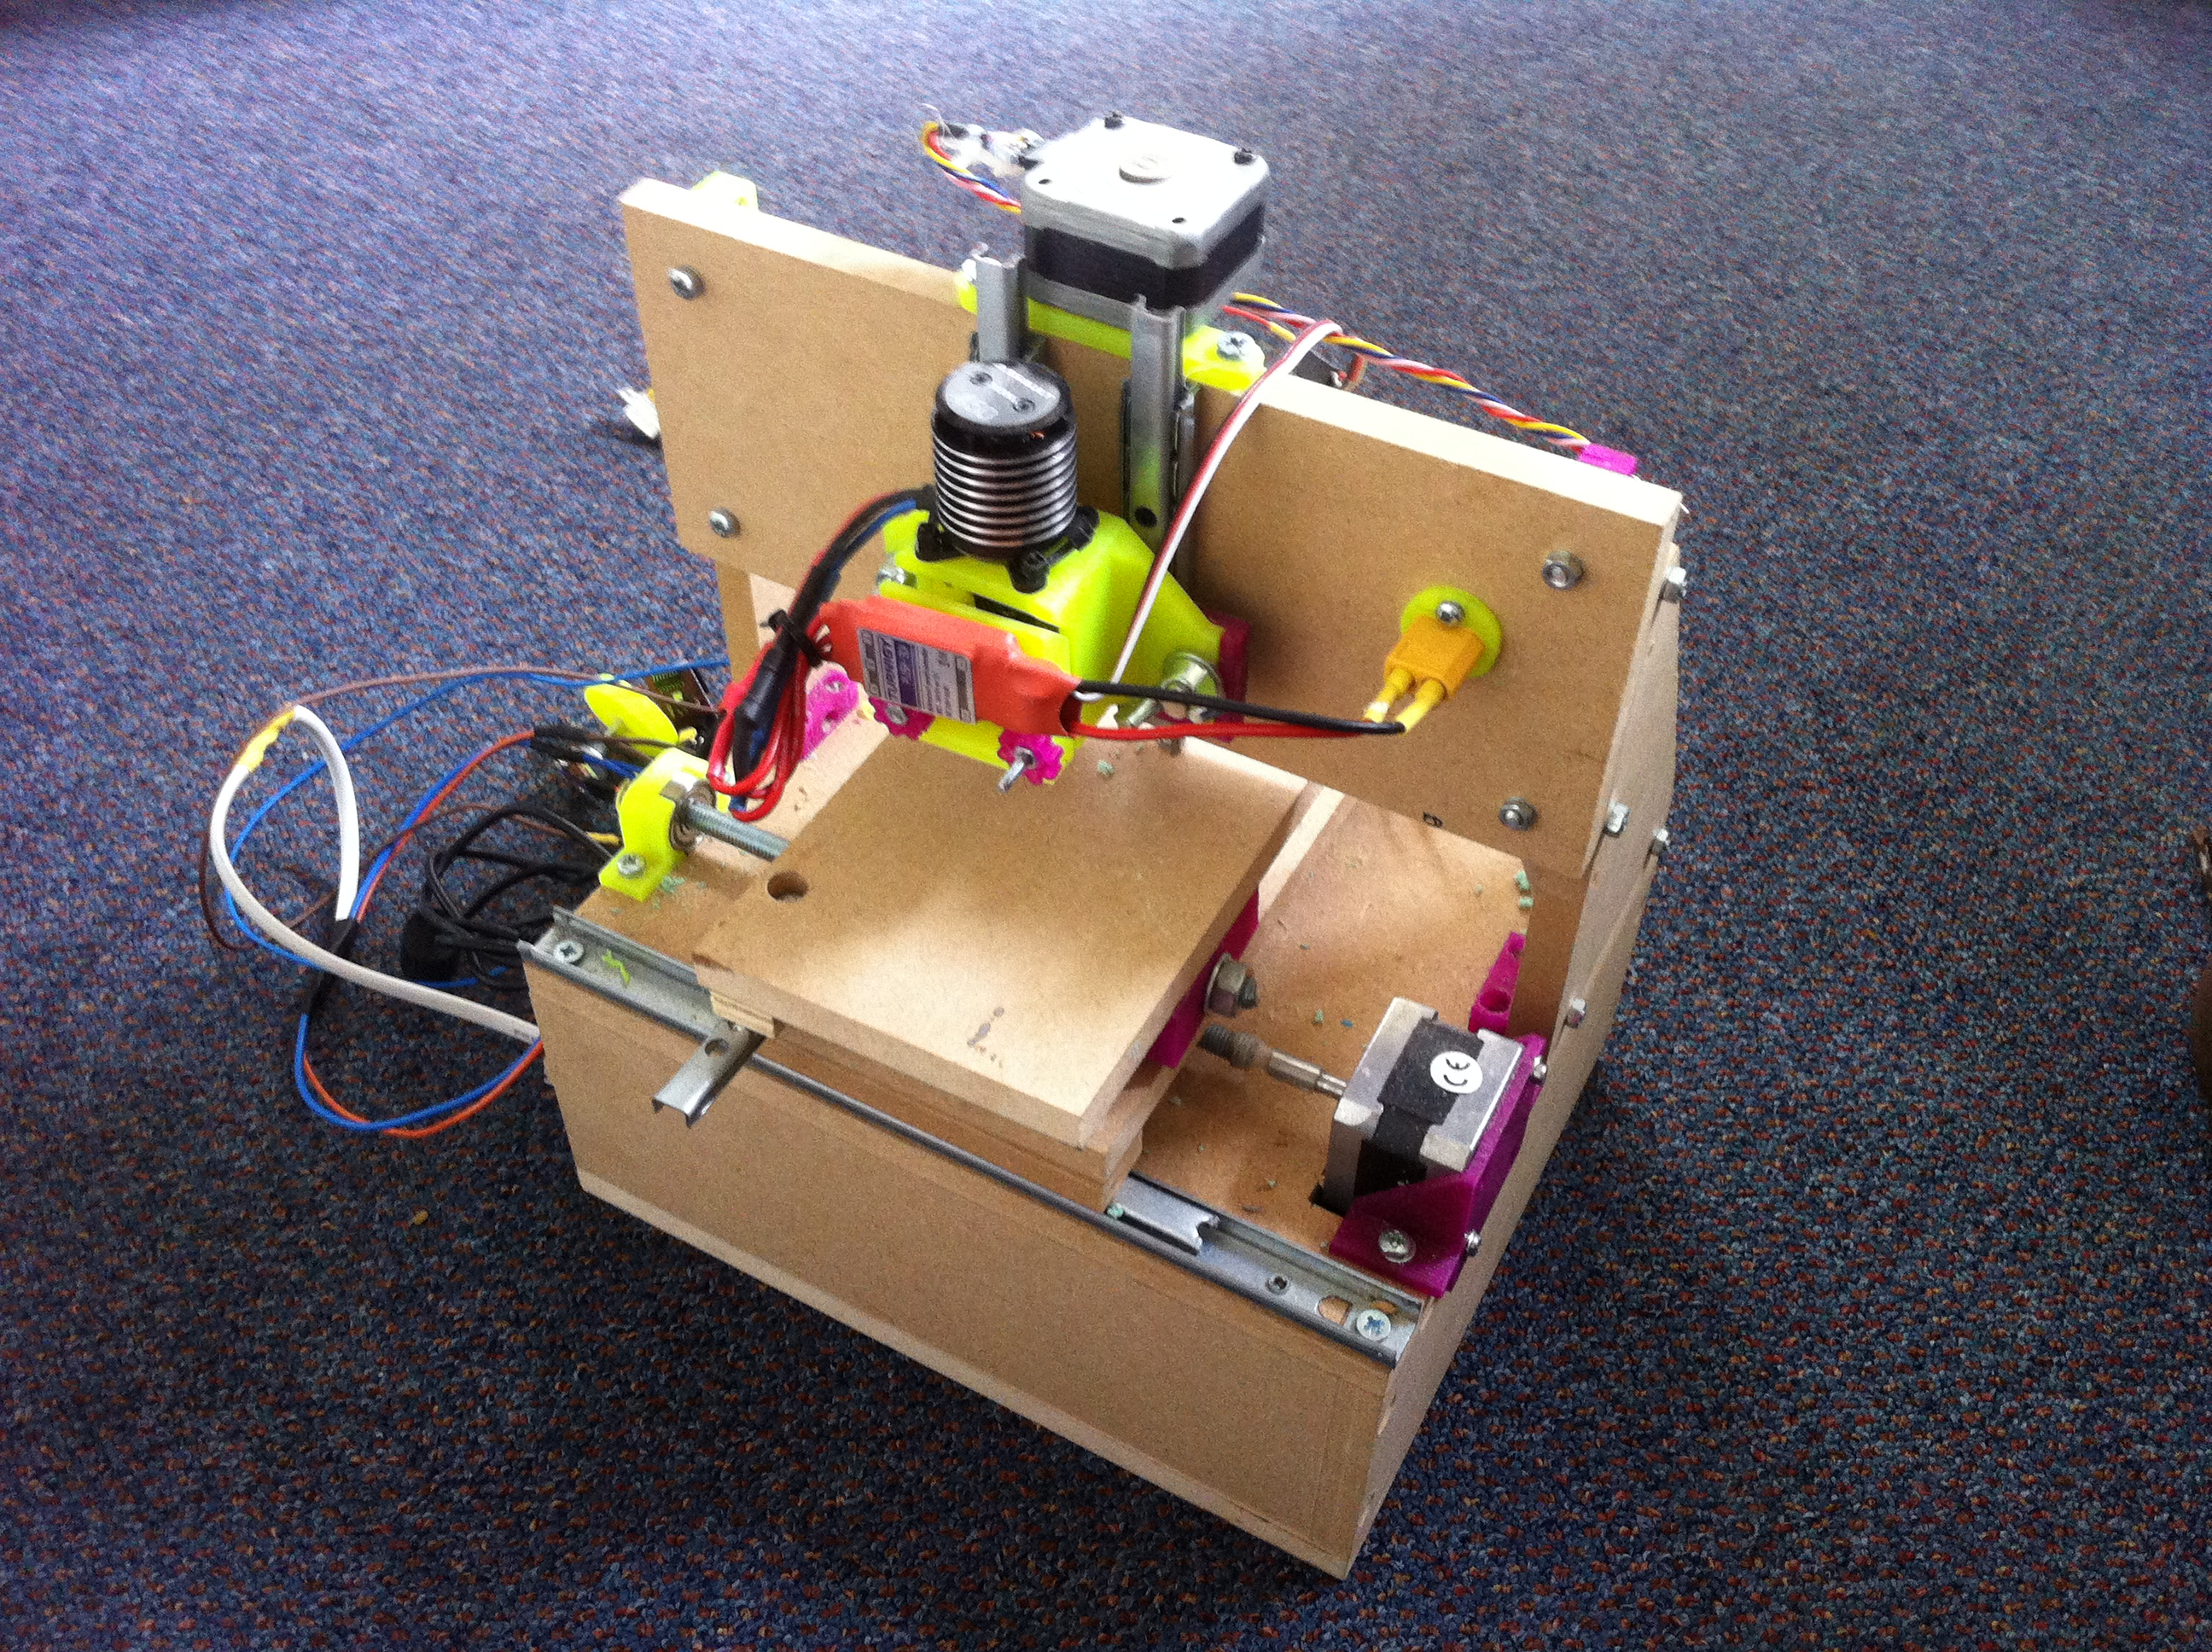
\includegraphics[width=160mm]{resources/finished.jpg}
\caption{Finished wooden version of the machine.}
\label{fig:finished}
\end{figure}


\newpage
\appendix
\appendixpage
\addappheadtotoc
\section{Servo tester}

\begin{figure}[ht!]
\centering
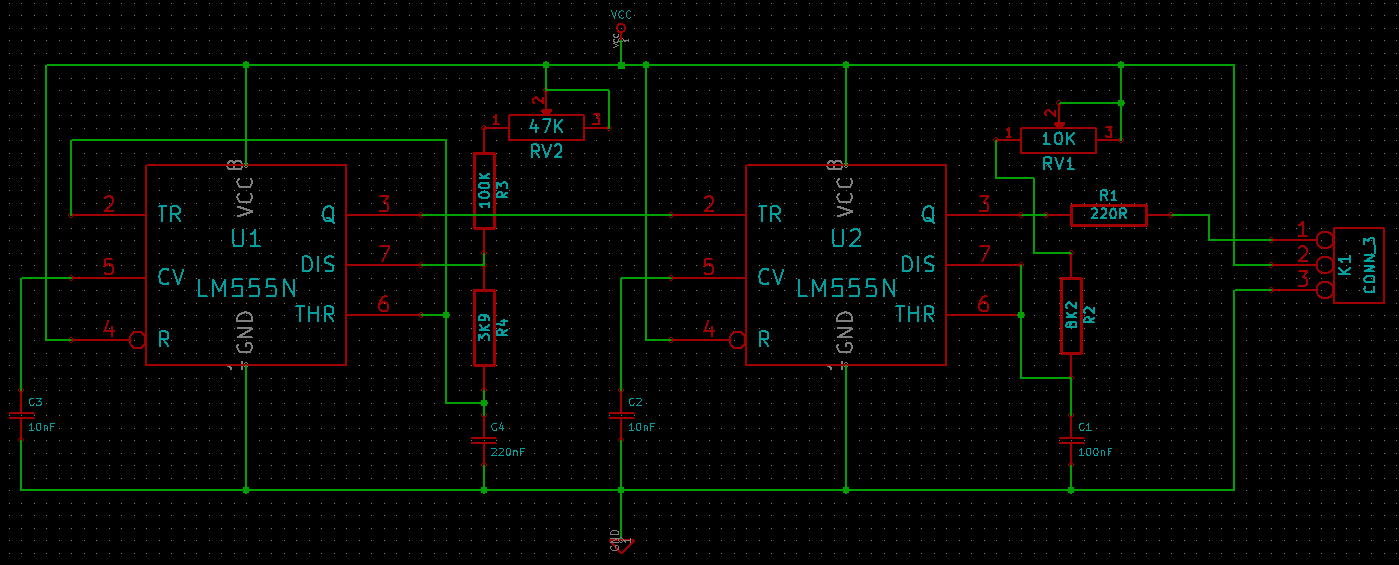
\includegraphics[width=160mm]{resources/servoexerciser.png}
\caption{Servo tester schematic.}
\label{fig:servotesterschem}
\end{figure}

The ESC used to control the brushless spindle motor is controlled with standard "servo" control. This consists of variable length pulses sent approximately 20ms apart.
The length of pulses corresponds to the position of the servo, or in this case the desired operation speed of the brushless motor. The pulses are specified to be 1-2ms,
which correspond to the minimum and maximum desired speeds.

During testing it because apparent that it would be useful to have manual control of spindle speed. A simple circuit was designed to provide the necessary pulses (See Figure \ref{fig:servotesterschem}).

The circuit works by using one 555 timer to generate a square wave of approximately 50Hz. This triggers a second 555 timer, which operates in monostable mode, with a pulse length
that is dependent on the position of a potentiometer. The 50Hz wave satisfies the condition of pulses that should be sent approximately every 20ms, and the pulses are varied between 1-2ms. The speed controllers
contain a 5V linear regulator which is connected to one pin of the servo connection. This powers the 555 timers so that no other power supply is required for operation. The circuit performed as expected and 
has been useful in project development.

\begin{figure}[ht!]
\centering
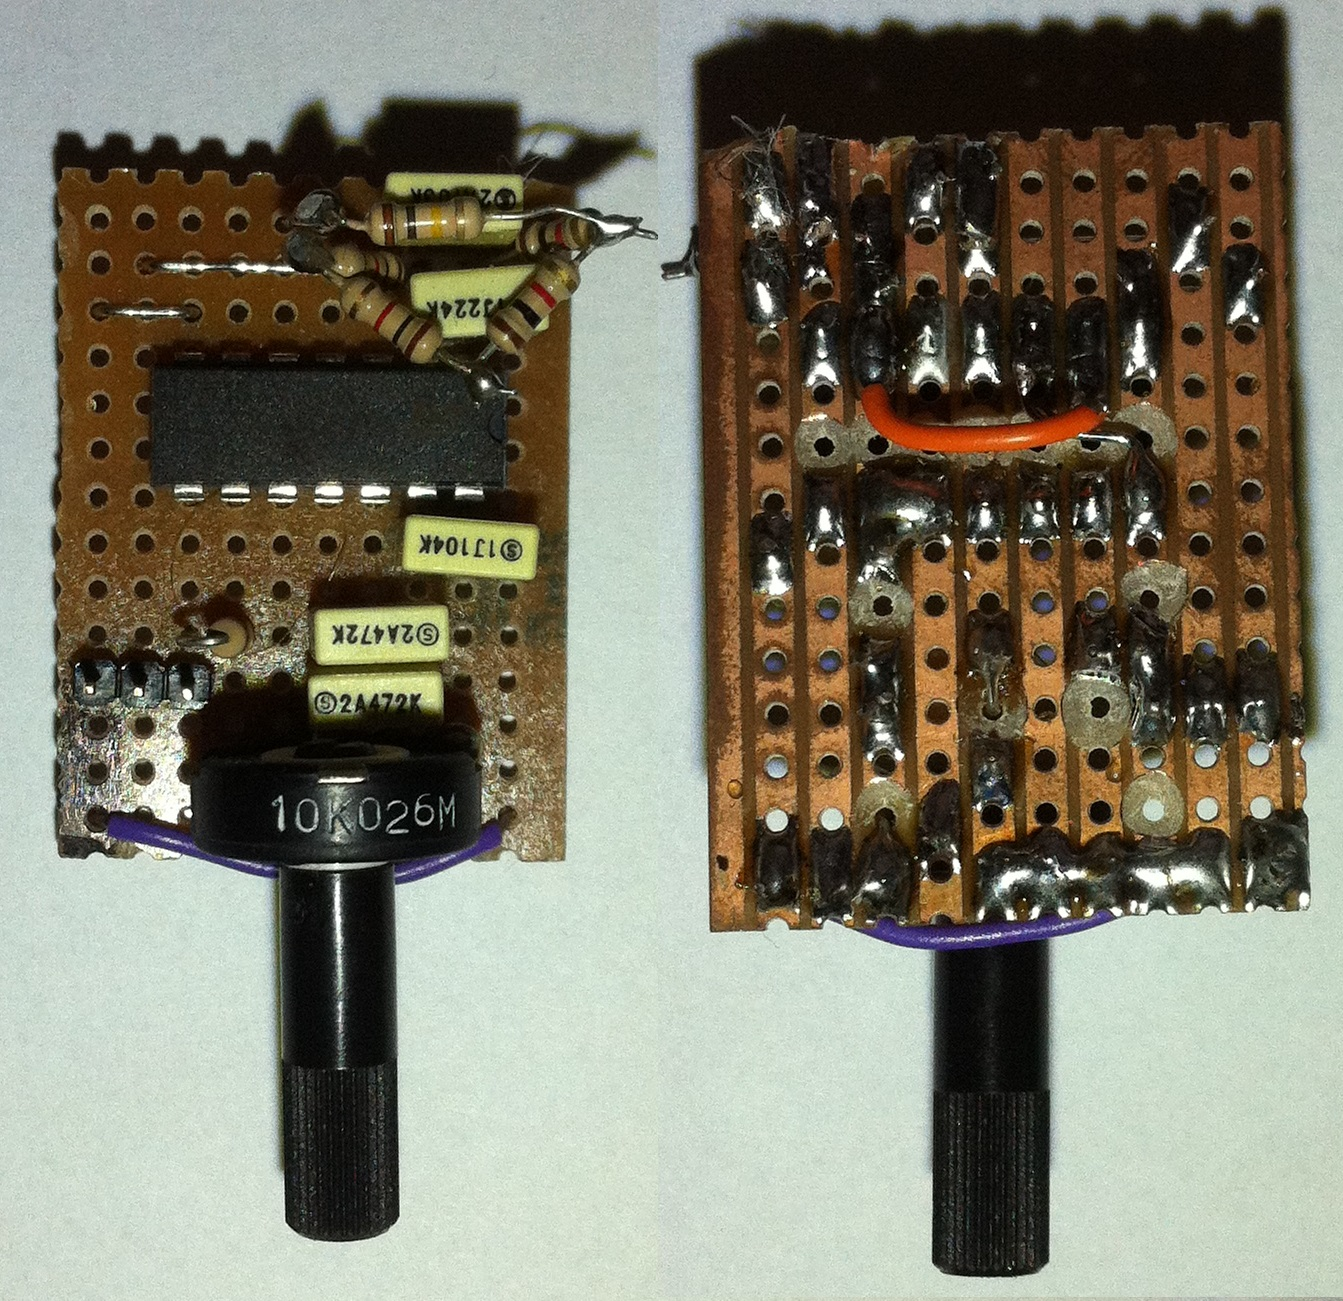
\includegraphics[width=90mm]{resources/servotester.jpg}
\caption{Servo tester board (front and back).}
\label{overflow}
\end{figure}

\newpage
\section{Calliper serial output modification}

\begin{figure}[ht!]
\centering
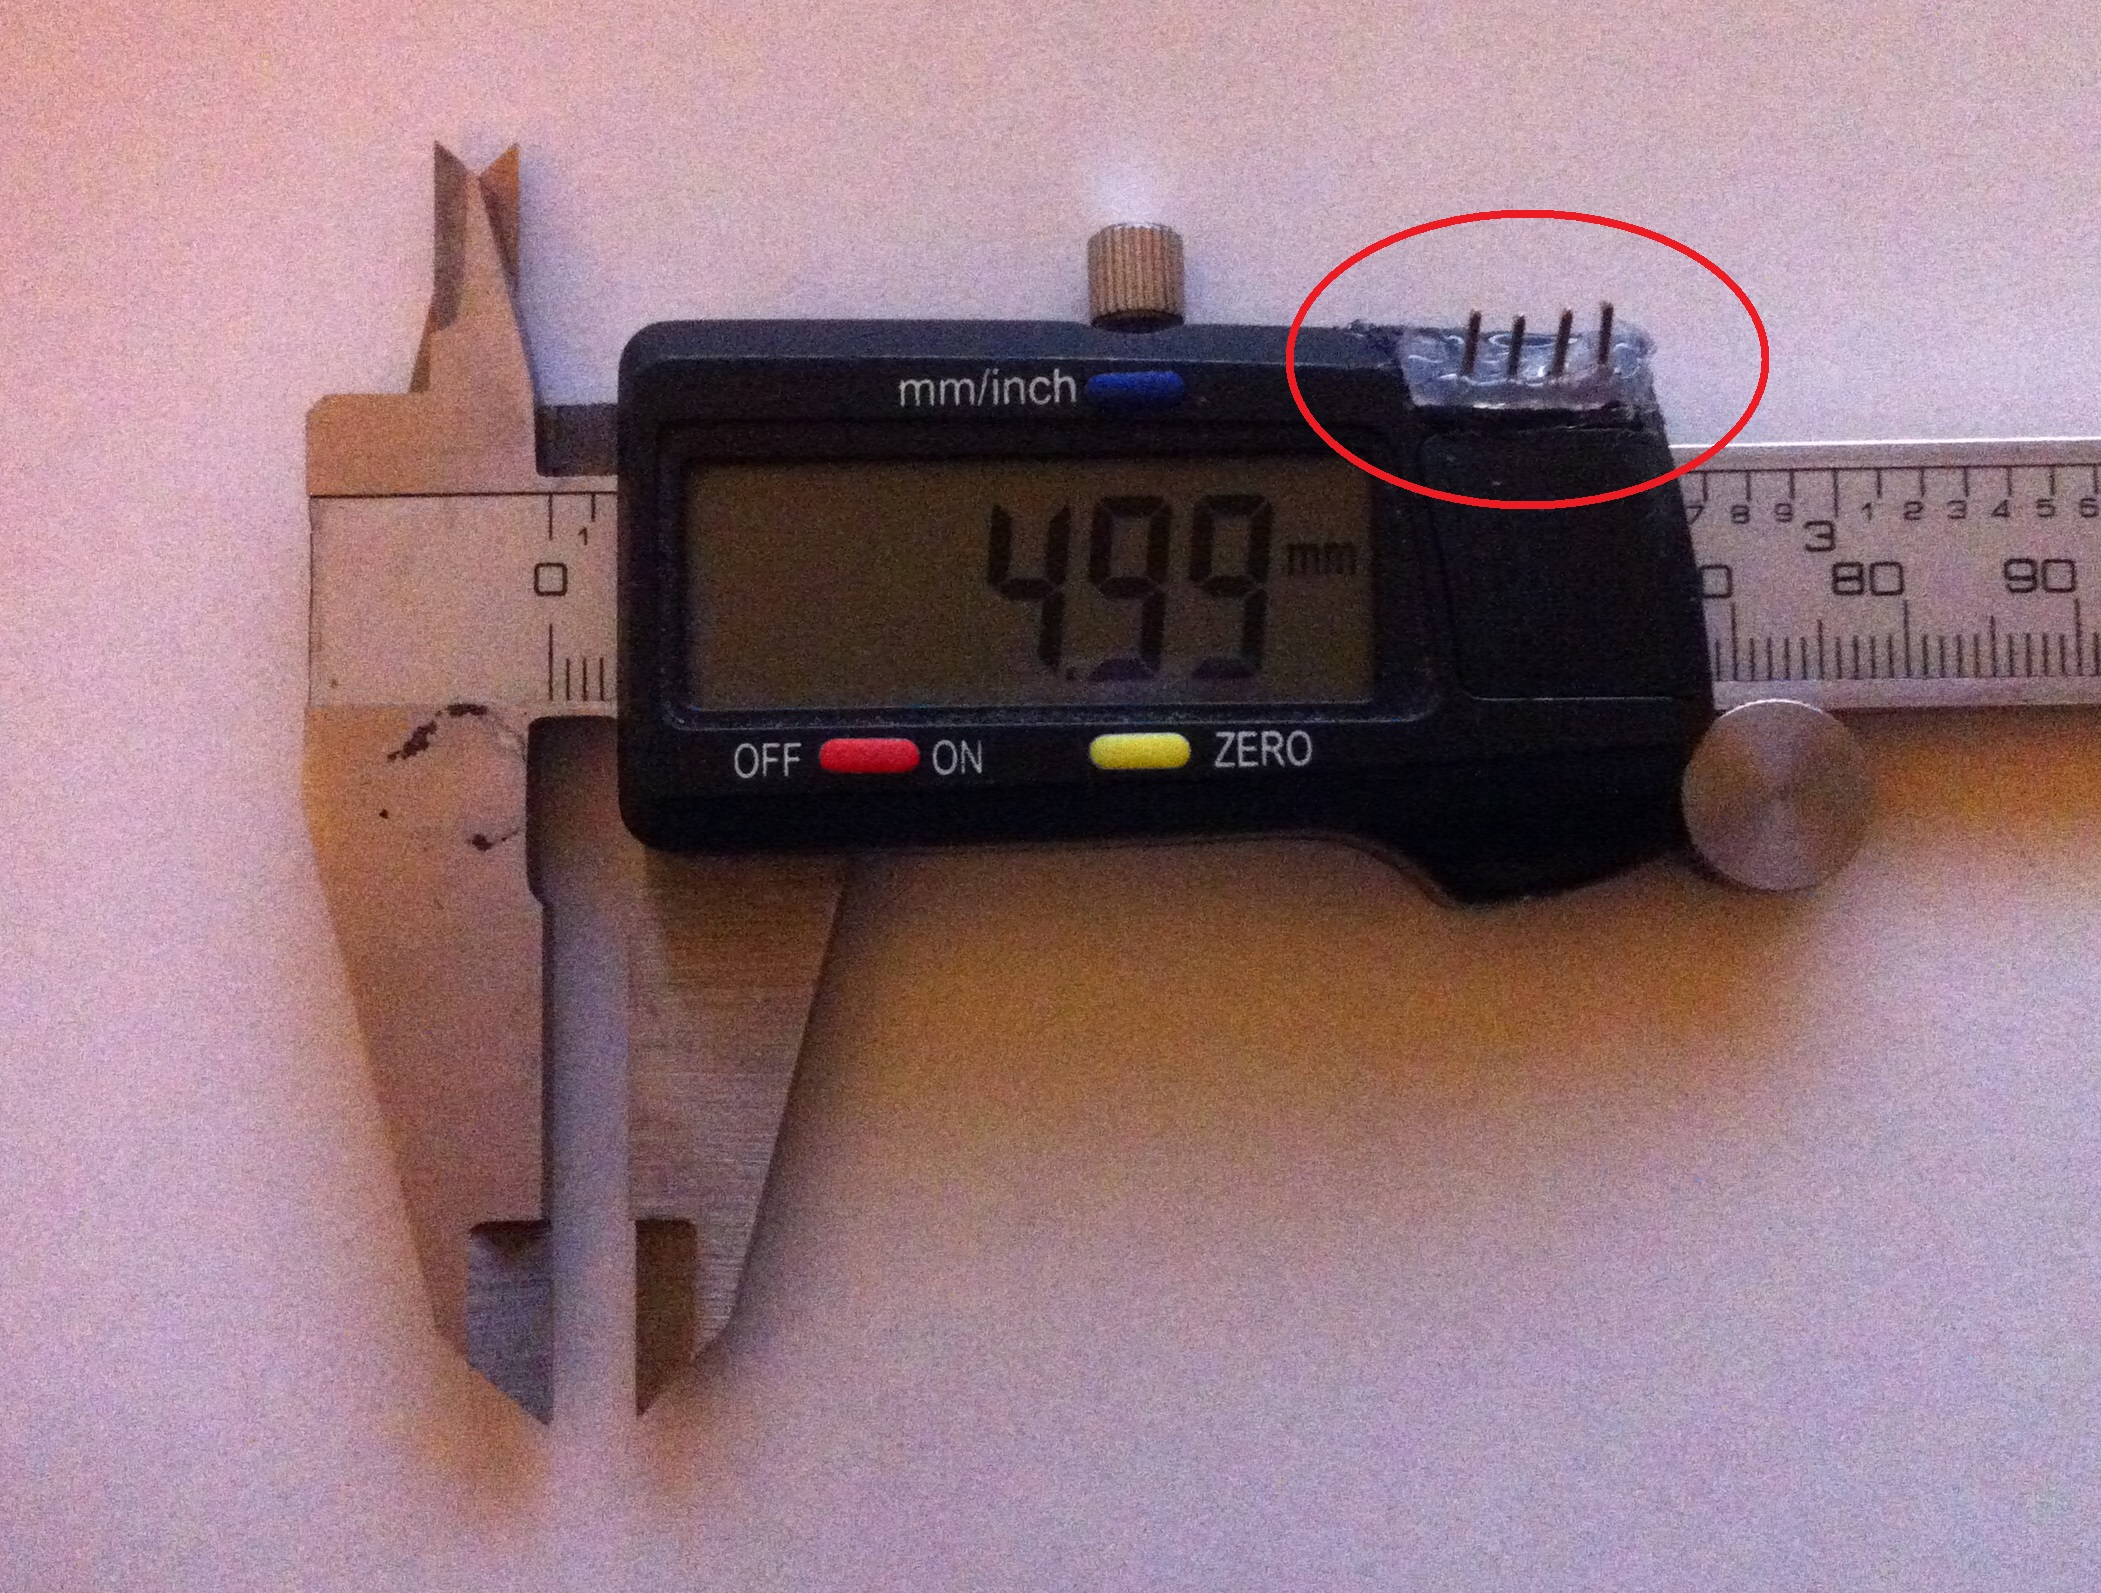
\includegraphics[width=150mm]{resources/callipermod.jpg}
\caption{Modified callipers (Data port highlighted in red).}
\label{overflow}
\end{figure}

During the testing of accuracy it was necessary to take a large number of positional measurements in all directions. 
To speed up this process, an inexpensive pair of callipers was modified to output a serial data stream which could be logged
against the position according to the firmware. Instructions located here: \cite{caliperdata}.

The positional data can be read from four traces on the calliper internal PCB. For convenience, the +V, ground, data and clock lines
were brought out on to four 2.54" pin headers. As the callipers are powered by a 1.5V battery, NPN transistors are used to amplify the signals to 5V. An ATTINY2313
decodes the data stream and converts it to a serial stream, sent via a USB-serial cable to the PC.

\newpage
\section{SMD component types}

A large variety of SMD types and sizes are available. A selection is described here (from \cite{smdwiki})

\subsection{Two-terminal passive components (mostly resistors and capacitors)}
Package types are given a four digit code, which describes the length and width in mm.

Example:

0603 is a 0.6 x 0.3mm rectangular package.

\subsection{SOT: Small-Outline Transistor}
Despite the name, these devices are not limited to single transistors, other types (eg linear regulators) are
common in the same packages.

Example:

SOT-223 is a 6.7x3.7x1.8mm body, three terminals plus a heat transfer pad.

\subsection{SOIC: Small-Outline Integrated Circuit}
Dual-in-line devices with 8 or more gull-wing lead form pins, spacing of 1.27mm

\newpage
\section{Part List}

Auto-generated from "Part List.xlsx" using \cite{excel2latex}.

\begin{tabular}{ | l | l | l | l | }
\hline
	Part & Number required & Total Cost & Supplier \\ \hline
	base\_board & 1 & - & - \\ \hline
	topboard & 1 & - & - \\ \hline
	bed & 1 & - & - \\ \hline
	zsupport & 2 & - & - \\ \hline
	zpanel & 1 & - & - \\ \hline
	base\_back & 1 & - & - \\ \hline
	base\_sides & 2 & - & - \\ \hline
	base\_bottom & 1 & - & - \\ \hline
	electronics\_tray & 1 & - & - \\ \hline
	drawer slides & 6 & 8 & \  \\ \hline
	m8 threaded rods & 3 & \  & \  \\ \hline
	m8 brass nuts & 6 & \  & \  \\ \hline
	anti-backlash springs & 3 & \  & \  \\ \hline
	electronics board & 1 & 30 & \  \\ \hline
	nema17 motors & 3 & 18 & Zapp Automation \\ \hline
	Vacuum tube & 1 & 1 & \  \\ \hline
	Turnigy plush 30A & 1 & 8 & Hobbyking \\ \hline
	Turnigy 450 3800KV & 1 & 8.56 & Hobbyking \\ \hline
	prop savers & 2 & 1.84 & Hobbyking \\ \hline
	m4 nuts and bolts & 40 & \  & \  \\ \hline
	12v 30A psu & 1 & 23.58 & \  \\ \hline
	nuttrap & 3 & \  & \  \\ \hline
	motorholder & 3 & \  & \  \\ \hline
	pasteextruder & 1 & \  & \  \\ \hline
	needleholder & 1 & \  & \  \\ \hline
	zholder & 1 & \  & \  \\ \hline
	rightangle & 4 & \  & \  \\ \hline
\end{tabular}




\newpage
\section{Improvements to report}
Need to do:

Get up to date render of machine for start of report.

\printglossaries

\nocite{*}
\printbibliography

\end{document}
